\section{Demo minh họa}
\label{sec:demo}

\subsection{Tổng quan thực nghiệm}
\label{subsec:tong-quan-thuc-nghiem}

Chương này trình bày ba demo tương tác được xây dựng để minh chứng thực nghiệm cho các phân tích lý thuyết ở Chương~\ref{sec:phuong-phap}. Mỗi demo đại diện cho một kiểu dữ liệu hình học và một cách tiếp cận khác nhau để đưa đối xứng vào mô hình: ảnh hai chiều chịu tác động của phép xoay, đám mây điểm ba chiều chịu tác động của phép hoán vị thứ tự điểm, và phân tử hóa học ba chiều đòi hỏi tính bất biến theo nhóm Euclidean $E(3)$. Mục tiêu chính không chỉ là báo cáo độ chính xác, mà còn là quan sát cách hành vi của mô hình thay đổi khi ta đưa trực tiếp inductive bias hình học vào dữ liệu hoặc kiến trúc.

\begin{table}[H]
\centering
\small
\renewcommand{\arraystretch}{1.2}
\begin{tabularx}{\textwidth}{p{0.18\textwidth}>{\raggedright\arraybackslash}X>{\raggedright\arraybackslash}X>{\raggedright\arraybackslash}X}
\toprule
& \textbf{Demo Part 1} & \textbf{Demo Part 2} & \textbf{Demo Part 3} \\
\midrule
Bài toán       & Phân loại chữ số viết tay    & Phân loại đám mây điểm 3D & Dự đoán năng lượng phân tử \\
Dữ liệu       & MNIST ($28\times28$, 10 lớp) & 5 lớp trích từ ModelNet40, 1024 điểm/mẫu & Tập con QM9 gồm 1000 phân tử \\
Nhóm đối xứng  & $SO(2)$, phép xoay trong mặt phẳng & $S_n$, phép hoán vị thứ tự điểm & $E(3)$, nhóm Euclidean trong $\mathbb{R}^3$ \\
Số mô hình     & 3 mô hình CNN & 2 biến thể PointNet & 2 cấu hình NequIP ($\ell=0$ và $\ell=1$) \\
Phương pháp    & Baseline, Data Augmentation, Frame Averaging & Shared MLP, max pooling, T-Net & Equivariant message passing với irrep \\
Liên kết lý thuyết & Mục~\ref{subsec:off-the-shelf} & Mục~\ref{sec:pointnet-paper} & Mục~\ref{subsec:nequip-paper} \\
\bottomrule
\end{tabularx}
\caption{Tổng quan ba demo thực nghiệm và liên kết với các phân tích lý thuyết trong đồ án.}
\label{tab:demo-overview}
\end{table}

Hệ thống demo được triển khai dưới dạng ứng dụng web gồm hai thành phần chính. \textit{Frontend} sử dụng Next.js, TypeScript, Tailwind CSS và Three.js để cung cấp giao diện vẽ chữ số, thanh trượt góc xoay, bộ chọn lớp vật thể và trình quan sát point cloud 3D. \textit{Backend} sử dụng FastAPI và PyTorch để phục vụ inference cho cả hai bài toán. Các mô hình được nạp một lần khi server khởi động và được giữ trong bộ nhớ trong suốt phiên chạy.

Cấu trúc thư mục thực tế trong repository được sử dụng như sau:

\begin{itemize} [leftmargin=2cm]
    \item \texttt{frontend/}: mã nguồn giao diện web.
    \item \texttt{backend/services/model\_service.py}: logic inference cho demo MNIST xoay.
    \item \texttt{backend/services/pointnet\_service.py}: logic inference cho demo PointNet.
    \item \texttt{backend/services/qm9\_service.py}: xây dựng đồ thị phân tử đầu vào cho NequIP.
    \item \texttt{backend/core/nequip\_wrapper.py}: tải và chạy checkpoint NequIP.
    \item \texttt{backend/api/part1\_routes.py}: endpoint \texttt{/api/part1/predict} phục vụ demo nhận diện chữ số MNIST.
    \item \texttt{backend/api/part2\_routes.py}: các endpoint \texttt{/api/part2/classify}, \texttt{/api/part2/sample/\{class\}} và \texttt{/api/part2/classes} phục vụ demo PointNet.
    \item \texttt{backend/api/part3\_routes.py}: endpoint \texttt{/api/part3/predict-energy} phục vụ demo dự đoán năng lượng NequIP.
    \item \texttt{backend/core/}: định nghĩa kiến trúc \texttt{SimpleCNN}, \texttt{FrameAveragingCNN}, \texttt{PointNetBasic} và \texttt{PointNetFull}.
    \item \texttt{storage/weights/}: các file trọng số cho Part 1 và Part 2.
    \item \texttt{ai\_core/outputs/nequip\_l1\_1000/best.ckpt}: checkpoint NequIP tốt nhất được triển khai trong demo.
    \item \texttt{ai\_core/outputs/}: bốn thư mục kết quả huấn luyện: \texttt{baseline\_l0\_100}, \texttt{baseline\_l0\_1000}, \texttt{nequip\_l1\_100} và \texttt{nequip\_l1\_1000}.
    \item \texttt{ai\_core/configs/}: bốn file cấu hình Hydra tương ứng với từng thực nghiệm.
    \item \texttt{ai\_core/notebooks/01\_mnist\_rotation\_invariance.ipynb}: notebook huấn luyện và đánh giá độ bền xoay cho Part 1.
    \item \texttt{ai\_core/notebooks/02\_modelnet\_pointcloud\_classification.ipynb}: notebook huấn luyện PointNet và trực quan hóa critical points cho Part 2.
    \item \texttt{ai\_core/notebooks/03\_qm9\_molecular\_energy\_prediction.ipynb}: notebook phân tích kết quả ablation NequIP và vẽ learning curve cho Part 3.
    \item \texttt{ai\_core/notebooks/nequip\_learning\_curve.py}: tiện ích vẽ đường cong học từ các checkpoint thực nghiệm.
\end{itemize}

Các thí nghiệm được thiết kế để có thể chạy trên CPU. Với quy mô demo hiện tại, việc dùng CPU giúp quá trình cài đặt và trình diễn đơn giản hơn, trong khi vẫn đủ để minh họa tác động của đối xứng lên hành vi mô hình. Các thư viện chính gồm PyTorch, torchvision, NumPy, Matplotlib, FastAPI và các thư viện frontend được khai báo trong \texttt{backend/requirements.txt} và \texttt{frontend/package.json}.

\subsection{Demo thực nghiệm Part 1: Nhận diện chữ số viết tay bất biến với phép xoay}
\label{subsec:demo-part1}

Demo đầu tiên hiện thực hóa bài toán phân loại chữ số viết tay trên giao diện web tương tác. Người dùng vẽ một chữ số trên canvas, điều chỉnh góc xoay, sau đó backend trả về đồng thời kết quả của ba mô hình: Baseline CNN, Augmented CNN và Frame Averaging CNN. Thiết kế này cho phép quan sát trực tiếp khác biệt giữa mô hình không có inductive bias hình học, mô hình học tính bất biến bằng data augmentation và mô hình ép tính bất biến bằng cơ chế frame averaging.

\begin{figure}[H]
\centering
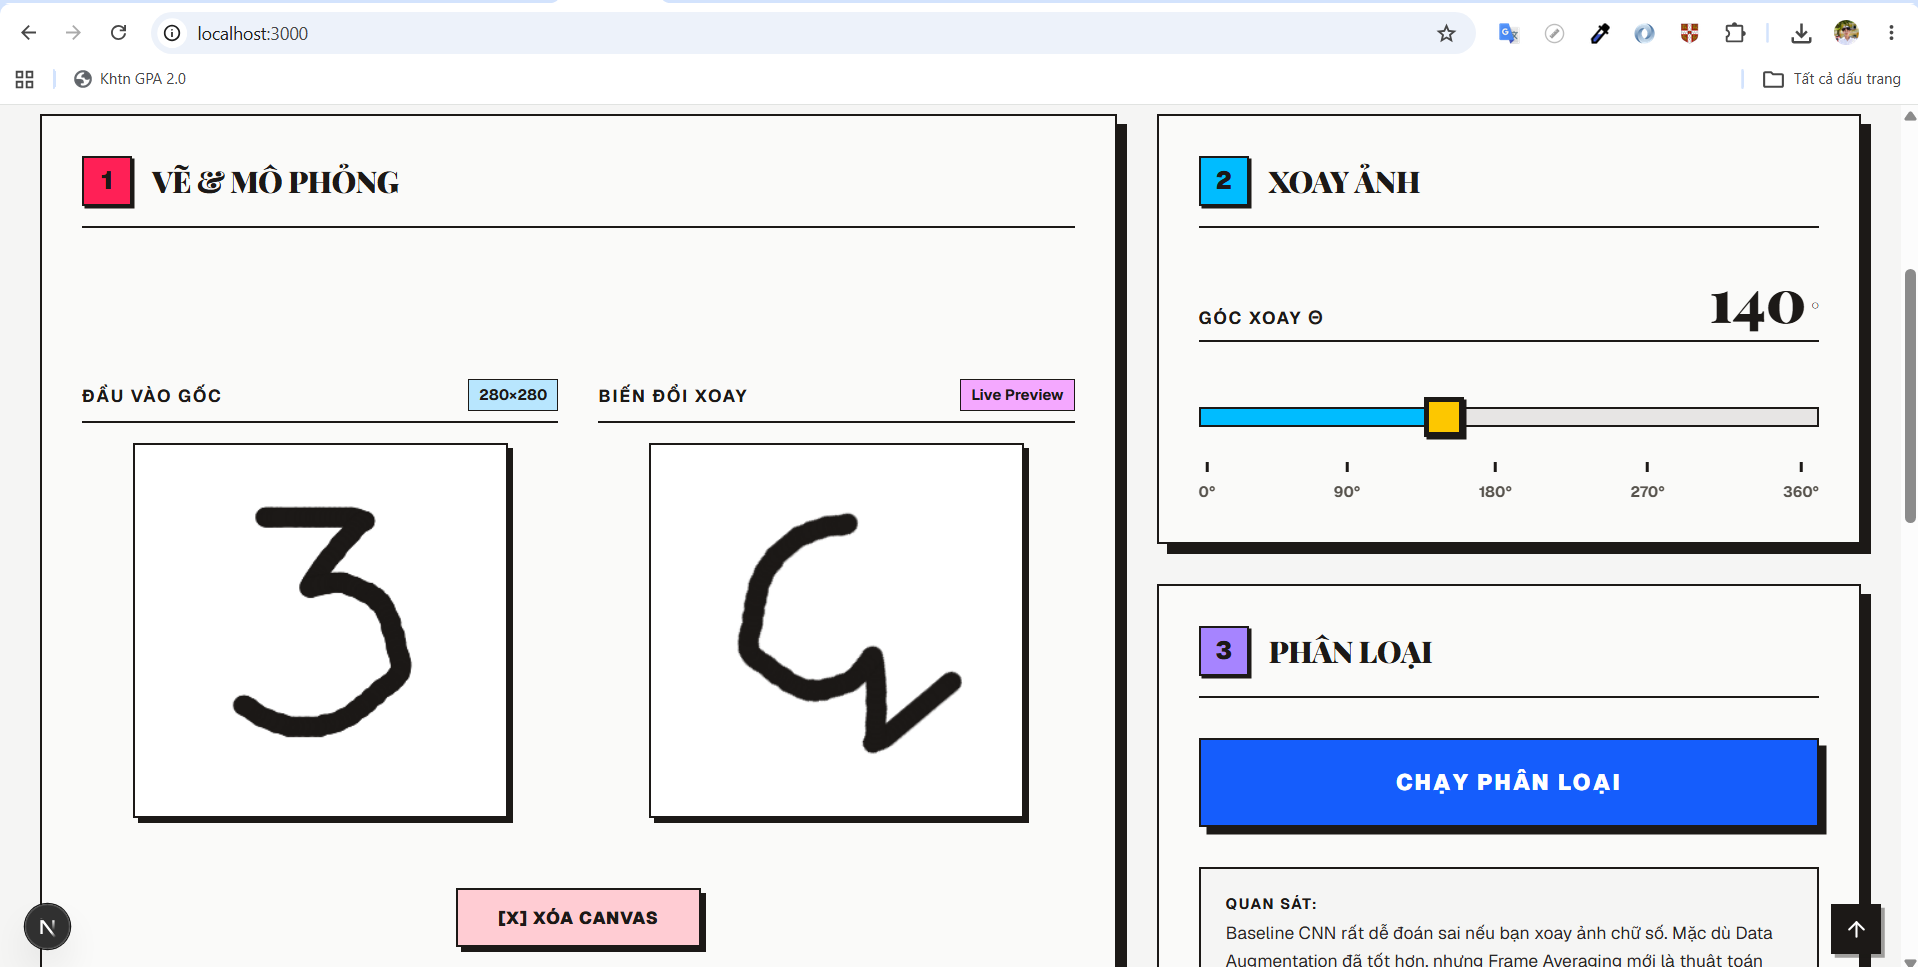
\includegraphics[width=0.90\textwidth]{graphics/web-p1.png}
\caption[Giao diện web demo nhận diện chữ số MNIST]{Giao diện demo Part 1.}
\label{fig:demo-part1-ui}
\end{figure}

\noindent\textit{Ghi chú: Người dùng vẽ chữ số vào ô số 1, điều chỉnh góc xoay bằng thanh trượt ở ô số 2 và quan sát mức độ tự tin của 3 thuật toán ở khung kết quả phía dưới.}

\subsubsection{Kiến trúc nền chung}

Ba mô hình dùng cùng một backbone CNN đơn giản để việc so sánh tập trung vào cách xử lý đối xứng thay vì sức mạnh kiến trúc:
\begin{equation}
\begin{aligned}
    &\mathrm{Conv}(1{\to}16, k=5) \to \mathrm{MaxPool}(2) \to
    \mathrm{Conv}(16{\to}32, k=5) \to \mathrm{MaxPool}(2) \\
    &\hspace{2.4cm}\to \mathrm{FC}(1568{\to}128) \to \mathrm{FC}(128{\to}10).
\end{aligned}
\label{eq:simplecnn-demo}
\end{equation}

Ảnh đầu vào được chuẩn hóa theo thống kê MNIST với $\mu=0.1307$ và $\sigma=0.3081$. Ở bước inference, backend cắt bounding box của nét vẽ, resize cạnh dài về 20 pixel bằng nội suy Lanczos, rồi căn \textit{center of mass} vào tâm ảnh $28\times28$. Quy trình này giúp dữ liệu do người dùng vẽ trên web gần hơn với phân phối MNIST gốc.

\subsubsection{Baseline CNN}

Mô hình Baseline được huấn luyện trên MNIST gốc, không áp dụng phép xoay trong quá trình load batch. Notebook \texttt{train\_models.ipynb} huấn luyện mô hình này trong 3 epoch, batch size 64. Loss trung bình in ra trong quá trình huấn luyện giảm từ khoảng 0.315 ở các batch đầu của epoch 1 xuống khoảng 0.034 ở cuối epoch 3. Điều này cho thấy mô hình học tốt phân phối MNIST thẳng đứng, nhưng không đồng nghĩa với việc mô hình đã học được tính bất biến với phép xoay.

Khi ảnh đầu vào bị xoay khỏi phân phối gốc, đặc biệt ở các góc lớn như $90^\circ$ hoặc $180^\circ$, dự đoán của Baseline dễ thay đổi mạnh. Đây là biểu hiện của việc mô hình phụ thuộc vào hướng xuất hiện trong dữ liệu huấn luyện. Nói cách khác, nếu không có inductive bias hình học, CNN thông thường không tự động suy ra rằng một chữ số sau khi xoay vẫn phải được xử lý theo một quy luật nhất quán.

\subsubsection{Augmented CNN}

Mô hình Augmented giữ nguyên kiến trúc ở phương trình~\eqref{eq:simplecnn-demo}, nhưng dữ liệu huấn luyện được biến đổi bằng phép xoay ngẫu nhiên:
\begin{equation}
    \texttt{RandomRotation}(180) \to \texttt{ToTensor}() \to \texttt{Normalize}(0.1307, 0.3081).
    \label{eq:mnist-augmentation-transform}
\end{equation}

Trong notebook, mô hình Augmented cũng được huấn luyện 3 epoch. Loss giảm từ khoảng 0.960 ở các batch đầu epoch 1 xuống khoảng 0.162 ở cuối epoch 3. So với Baseline, loss ban đầu cao hơn vì bài toán khó hơn: mô hình phải học chữ số trong nhiều tư thế khác nhau. Đổi lại, mô hình có khả năng ổn định hơn khi người dùng xoay ảnh đầu vào.

Tuy nhiên, data augmentation chỉ tạo ra tính bất biến ở mức xấp xỉ. Với một số cặp chữ số có hình dạng gần nhau sau khi xoay, chẳng hạn 6 và 9 ở góc $180^\circ$, bản thân nhãn trở nên mơ hồ. Trong trường hợp này, việc bổ sung thêm ảnh xoay không giải quyết triệt để vấn đề, vì cùng một hình dạng quan sát được có thể tương ứng với hai nhãn khác nhau tùy theo quy ước hướng ban đầu.

\subsubsection{Frame Averaging CNN}

Mô hình Frame Averaging sử dụng cùng backbone CNN, nhưng bọc bên ngoài bằng lớp \texttt{FrameAveragingCNN}. Cơ chế này dựa trên ý tưởng đã trình bày ở Mục~\ref{subsubsec:frame-averaging}: thay vì yêu cầu backbone tự học mọi góc xoay, ta xây dựng một tập khung gồm nhiều phiên bản đã căn chỉnh của đầu vào, đưa từng phiên bản qua backbone, sau đó lấy trung bình logits.

Bước đầu tiên là ước lượng hướng chính của nét chữ bằng PCA trên các điểm ảnh có giá trị lớn hơn ngưỡng:
\begin{equation}
    \Sigma = \frac{1}{|P|-1} \sum_{(x,y)\in P}
    \begin{pmatrix}x-\bar{x}\\y-\bar{y}\end{pmatrix}
    \begin{pmatrix}x-\bar{x}\\y-\bar{y}\end{pmatrix}^{\!\top},
    \qquad
    P = \{(x,y): I(x,y) > 0.2\}.
    \label{eq:mnist-pca-covariance}
\end{equation}

Sau đó, mô hình tạo bốn bản sao xoay lệch nhau $90^\circ$:
\begin{equation}
    \mathcal{F}(I) = \{\mathrm{Rot}(I,-\theta_{\mathrm{PCA}} + k\cdot90^\circ) \mid k=0,1,2,3\}.
    \label{eq:mnist-frame-set}
\end{equation}

Logits cuối cùng được tính bằng trung bình cộng:
\begin{equation}
    \hat{y} = \frac{1}{4}\sum_{k=0}^{3} f_{\theta}\!\left(\mathrm{Rot}(I,-\theta_{\mathrm{PCA}} + k\cdot90^\circ)\right).
    \label{eq:mnist-frame-average-logits}
\end{equation}

Trong notebook, loss của mô hình Frame Averaging giảm từ khoảng 0.769 ở các batch đầu epoch 1 xuống khoảng 0.076 ở cuối epoch 3. Kết quả này cho thấy mô hình vẫn học ổn định dù phải xử lý nhiều phiên bản xoay của cùng một ảnh. So với Augmented CNN, điểm khác biệt quan trọng là tính bất biến được đưa vào quy trình suy luận bằng phép lấy trung bình trên frame, thay vì chỉ được hy vọng học thông qua dữ liệu xoay.
\begin{figure}[H]
\centering
\begin{tikzpicture}[>=Stealth, thick,
    box/.style={draw, rounded corners, minimum width=3.6cm, minimum height=1cm, font=\small, align=center, inner sep=6pt}]

    \node[box, fill=red!10]    (bl) at (0,0) {Baseline\\ \footnotesize Phụ thuộc hướng gốc};
    \node[box, fill=yellow!20] (au) at (5.5,0) {Augmentation\\ \footnotesize Bất biến xấp xỉ};
    \node[box, fill=green!15]  (fa) at (11,0) {Frame Averaging\\ \footnotesize Bất biến theo frame};

    \node[below=0.5cm of bl, font=\footnotesize, text=red!80!black] {$\theta$ lớn $\Rightarrow$ dễ sai};
    \node[below=0.5cm of au, font=\footnotesize, text=orange!90!black] {ổn định hơn, còn ambiguity};
    \node[below=0.5cm of fa, font=\footnotesize, text=green!70!black] {ổn định hơn khi xoay};

    \draw[->, dashed, gray!90!black] (bl.east) -- (au.west) node[midway, above, font=\footnotesize]{+data};
    \draw[->, dashed, gray!90!black] (au.east) -- (fa.west) node[midway, above, font=\footnotesize]{+frame};
\end{tikzpicture}
\caption{So sánh trực giác giữa ba hướng xử lý phép xoay trong demo MNIST.}
\label{fig:demo-part1-compare}
\end{figure}

\begin{table}[H]
\centering
\small
\renewcommand{\arraystretch}{1.3}
\caption{Tổng hợp đặc tính của ba mô hình trong demo Part 1.}
\label{tab:demo-part1-summary}
\begin{tabularx}{\textwidth}{@{} l c >{\raggedright\arraybackslash}X >{\raggedright\arraybackslash}X @{}}
\toprule
\textbf{Phương pháp} & \textbf{Thay đổi kiến trúc} & \textbf{Cách xử lý xoay} & \textbf{Ghi nhận chính} \\
\midrule
Baseline CNN & Không & Không xử lý trực tiếp & Tốt trên ảnh thẳng, yếu khi OOD theo góc \\
Augmented CNN & Không & Học từ ảnh xoay ngẫu nhiên & Ổn định hơn, nhưng chỉ là bất biến xấp xỉ \\
Frame Averaging CNN & Có wrapper & Trung bình trên 4 frame & Đưa đối xứng vào bước suy luận \\
\bottomrule
\end{tabularx}
\label{tab:demo-part1-summary}
\end{table}

\begin{figure}[H]
\centering
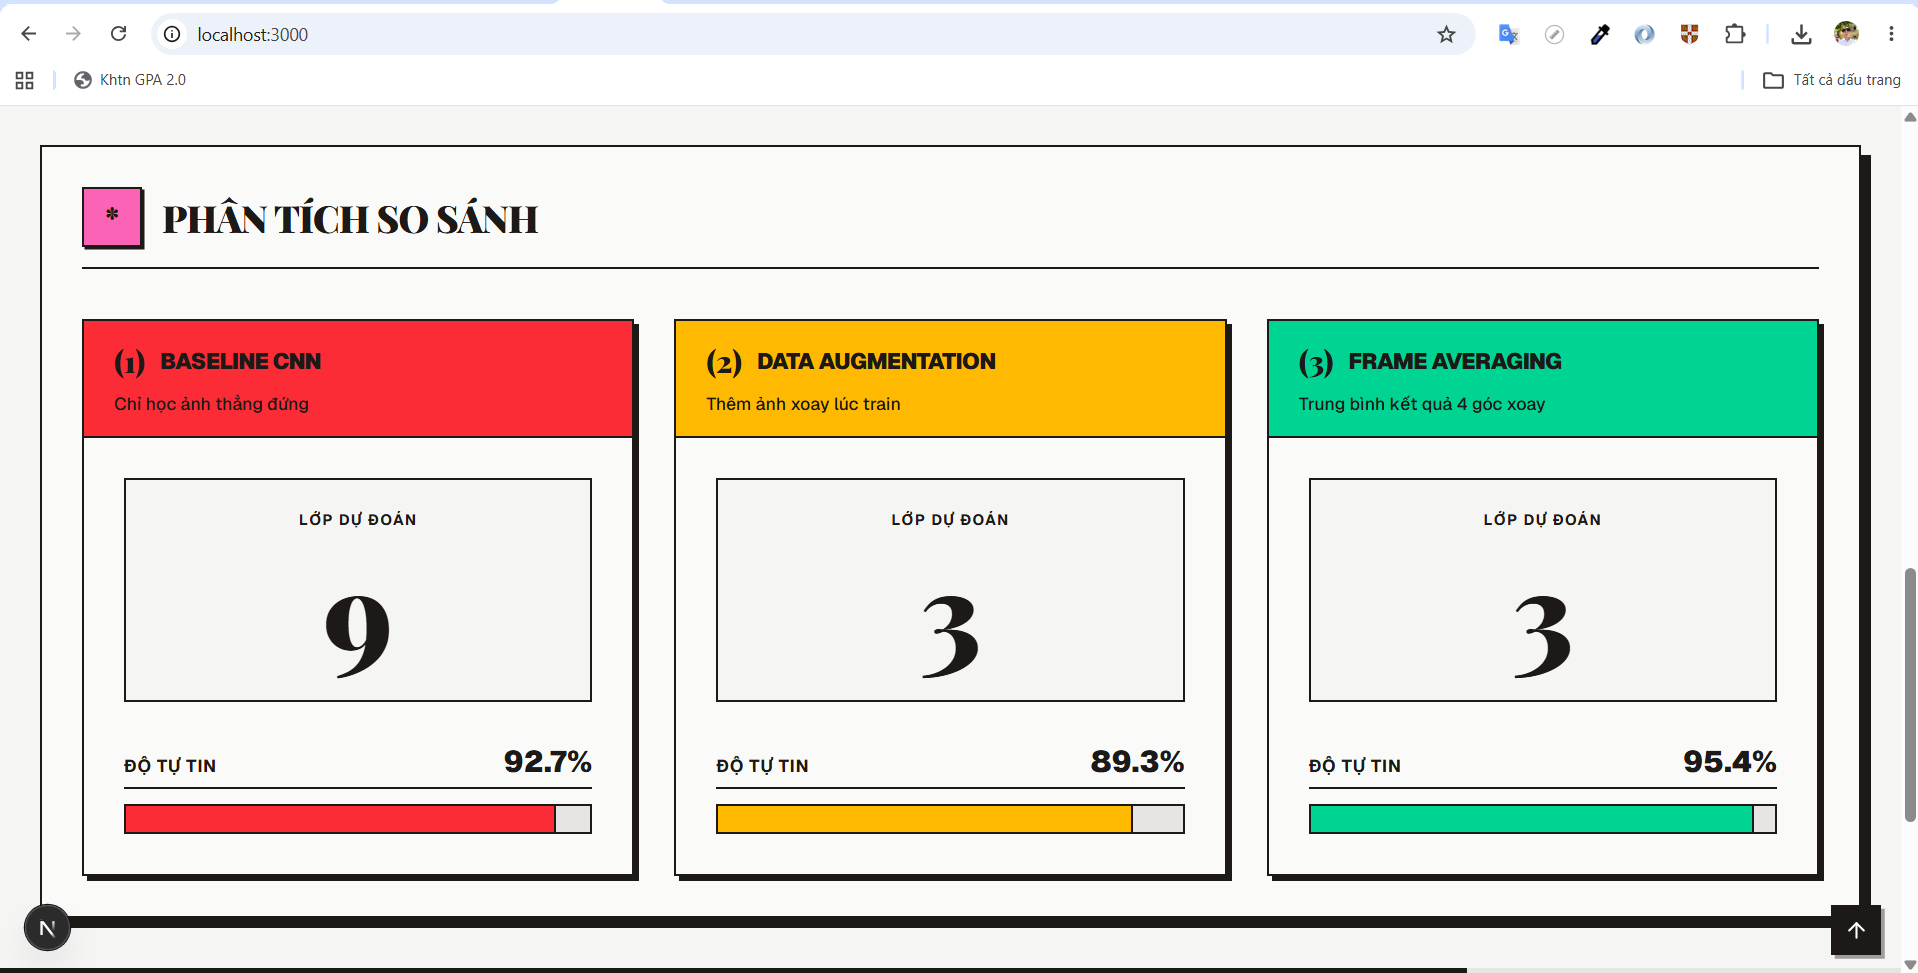
\includegraphics[width=0.90\textwidth]{graphics/demo_part1_result.png}
\caption{Kết quả phân tích độ tự tin của 3 mô hình trên giao diện web demo.}
\label{fig:demo-part1-result}
\end{figure}

\noindent\textit{Ghi chú: Khi người dùng xoay chữ số 3 với góc $140^\circ$, Baseline CNN dự đoán sai thành số 9 với 92.7\% độ tự tin. Mô hình Data Augmentation dự đoán đúng số 3 nhưng độ tự tin chỉ đạt 89.3\%. Trong khi đó, Frame Averaging thể hiện sự vượt trội khi dự đoán chính xác số 3 với độ tự tin cực đại lên tới 95.4\% nhờ cơ chế tính toán trung bình góc xoay.}

\subsection{Demo thực nghiệm Part 2: Phân loại đám mây điểm ba chiều với PointNet}
\label{subsec:demo-part2}

Demo thứ hai minh họa bài toán phân loại point cloud 3D. Người dùng chọn một trong năm lớp vật thể gồm \texttt{airplane}, \texttt{car}, \texttt{chair}, \texttt{lamp} và \texttt{table}. Sau đó có thể thay đổi số điểm đầu vào, thêm nhiễu Gaussian, xoay point cloud hoặc bỏ ngẫu nhiên một tỉ lệ điểm. Backend chạy đồng thời \texttt{PointNetBasic} và \texttt{PointNetFull}, sau đó trả về nhãn dự đoán, top 3 xác suất và tập critical points.

\begin{figure}[H]
\centering
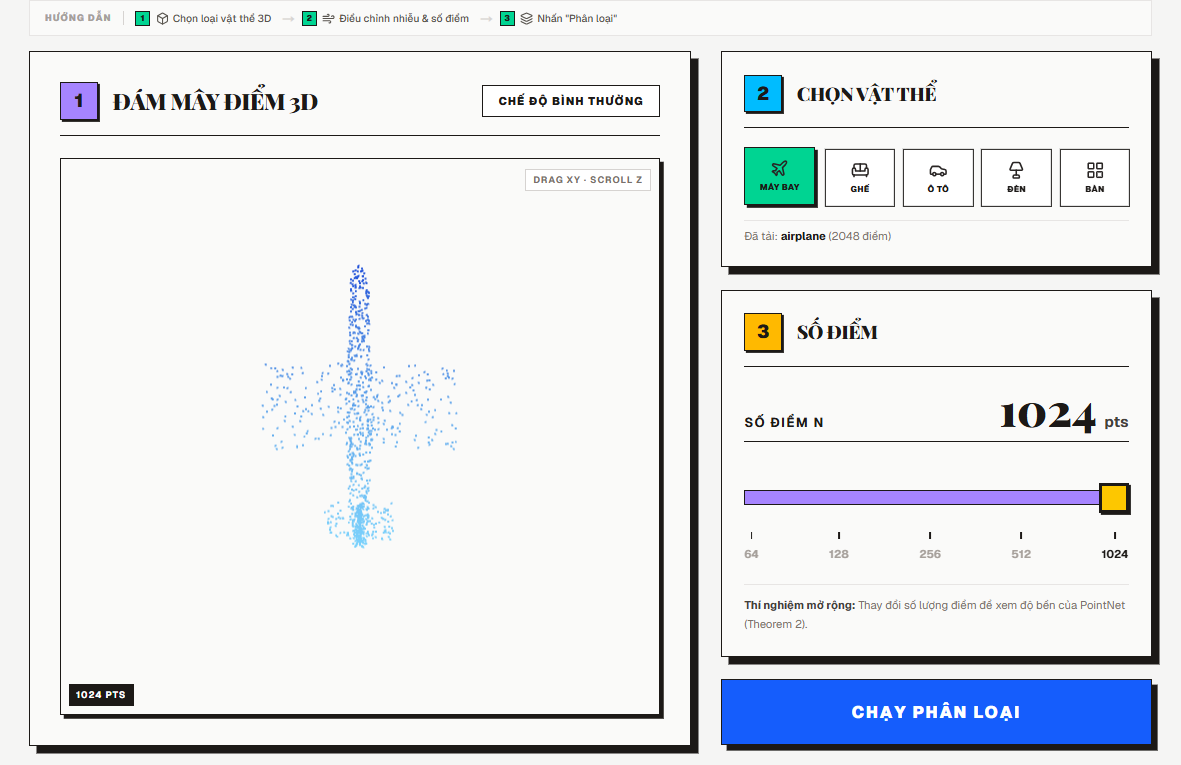
\includegraphics[width=0.90\textwidth]{graphics/fligt-1024pts.png}
\caption{Giao diện demo Part 2.}
\label{fig:demo-part2-ui}
\end{figure}

\noindent\textit{Ghi chú: Chọn vật thể máy bay, đặt số điểm là 1024 ở chế độ bình thường. Point cloud hiển thị trong viewer 3D và có thể kéo xoay tự do.}

\subsubsection{Dữ liệu và tiền xử lý}

Demo hiện tại sử dụng 5 lớp đại diện từ ModelNet40 thay vì toàn bộ 40 lớp. Đây là lựa chọn phù hợp với mục tiêu minh họa vì năm lớp này có hình dạng tương đối khác nhau, giúp người dùng quan sát rõ cơ chế hoạt động của PointNet mà không cần tải toàn bộ dataset lớn. Các point cloud mẫu được lưu tại \texttt{storage/data/sample\_clouds/} dưới định dạng \texttt{.npy}.

Trong notebook \texttt{pointnet\_classification.ipynb}, tập huấn luyện gồm 1000 mẫu, tương ứng 200 mẫu cho mỗi lớp và tập validation gồm 250 mẫu, tương ứng 50 mẫu cho mỗi lớp. Mỗi mẫu có 1024 điểm trong không gian ba chiều. Trước khi đưa vào mạng, point cloud được chuẩn hóa về hình cầu đơn vị:
\begin{equation}
    \tilde{P}_i = \frac{P_i - \bar{P}}{\max_j \|P_j - \bar{P}\|},
    \qquad
    \bar{P}=\frac{1}{n}\sum_{i=1}^{n}P_i.
    \label{eq:normalize-unit-sphere-demo}
\end{equation}

Bước này đưa point cloud về gốc tọa độ bằng cách trừ centroid, rồi thu về cùng tỉ lệ bằng cách chia cho khoảng cách điểm xa nhất. Nhờ vậy mô hình chỉ cần học hình dạng, không bị ảnh hưởng bởi vị trí hay kích thước ban đầu của vật thể.

\begin{figure}[H]
\centering
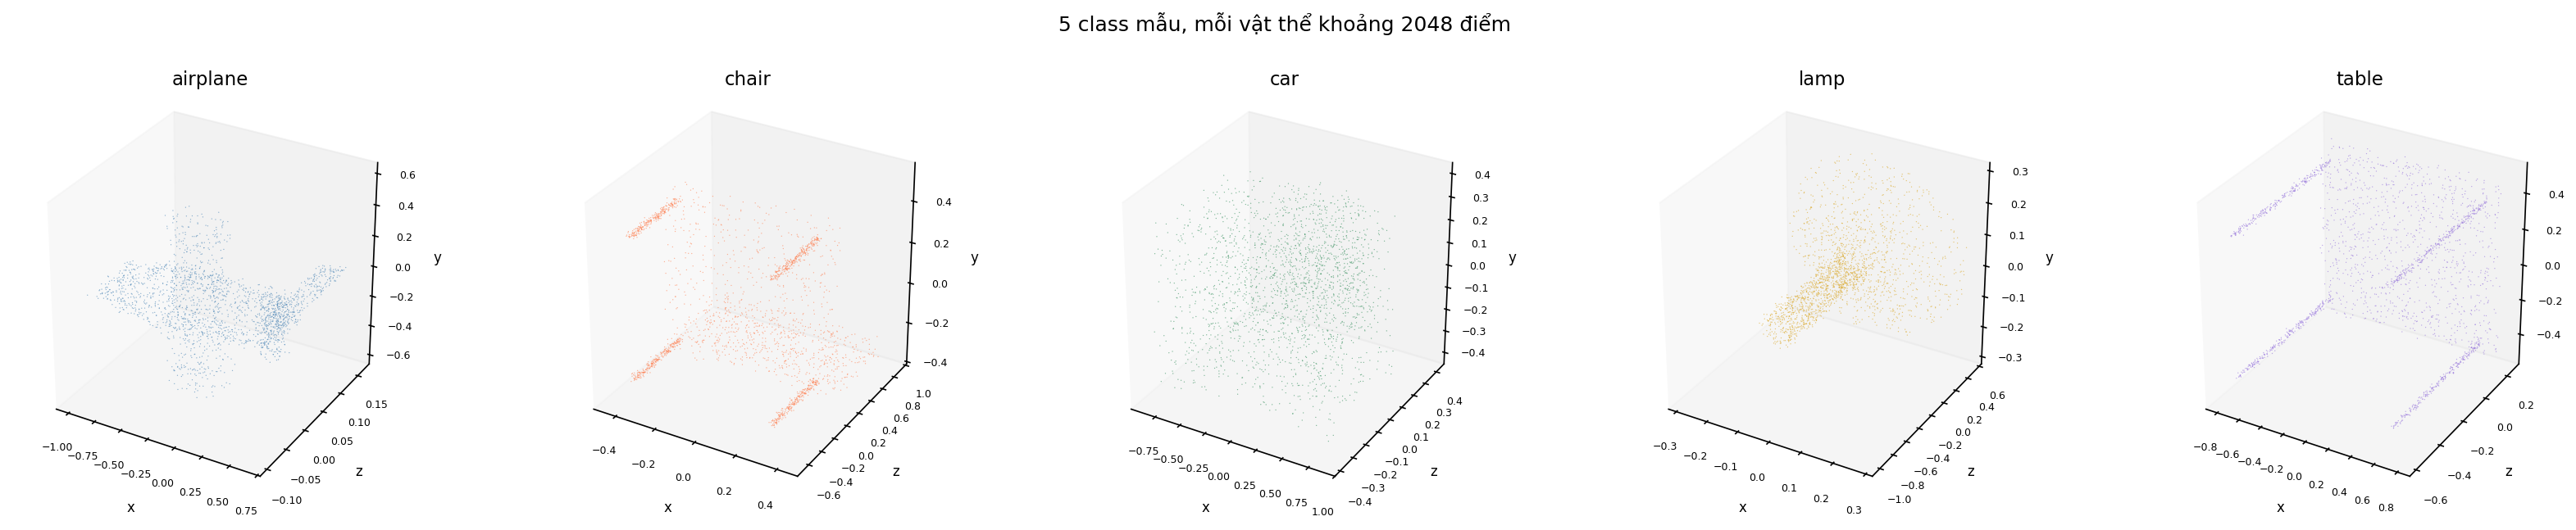
\includegraphics[width=0.78\textwidth]{graphics/point_clouds_5class_2.png}
\caption{Năm lớp point cloud được sử dụng trong demo Part 2.}
\label{fig:demo-point-clouds-5class}
\end{figure}

\subsubsection{Hai biến thể PointNet được so sánh}

\texttt{PointNetBasic} triển khai ý tưởng cốt lõi của PointNet: áp dụng shared MLP lên từng điểm độc lập, sau đó dùng global max pooling để gom toàn bộ tập điểm thành một vector đặc trưng toàn cục. Công thức tổng quát có thể viết dưới dạng:
\begin{equation}
    f(\{x_1,\ldots,x_n\}) \approx \gamma\!\left(\max_{i=1}^{n} h(x_i)\right),
    \label{eq:pointnet-approx-demo}
\end{equation}
trong đó $h$ là shared MLP xử lý từng điểm, $\max$ là hàm gộp không phụ thuộc thứ tự, và $\gamma$ là mạng phân loại phía sau. Vì phép max cho cùng kết quả dù điểm đầu vào được sắp xếp theo thứ tự nào, dự đoán của mô hình không thay đổi dù point cloud bị xáo trộn.

\texttt{PointNetFull} bổ sung hai T-Net. Input T-Net dự đoán ma trận $3\times3$ để căn chỉnh tọa độ đầu vào, còn Feature T-Net dự đoán ma trận $64\times64$ để căn chỉnh không gian đặc trưng. Khi huấn luyện, loss có thêm một số hạng phạt để buộc ma trận $A$ gần trực giao:
\begin{equation}
    \mathcal{L}=\mathcal{L}_{\mathrm{CE}} + \lambda\|I-AA^\top\|_F^2,
    \qquad \lambda=10^{-3},
    \label{eq:pointnet-full-loss-demo}
\end{equation}
trong đó $A$ là ma trận biến đổi do Feature T-Net dự đoán. Trong thiết lập demo, T-Net được giữ ổn định để tránh hiện tượng học không ổn định trên tập nhỏ.

Notebook ghi nhận số tham số của hai mô hình như sau: \texttt{PointNetBasic} có 810,629 tham số, còn \texttt{PointNetFull} có 3,471,054 tham số. Phần chênh lệch 2,660,425 tham số chủ yếu đến từ hai mạng T-Net.

\subsubsection{Thiết lập huấn luyện và kết quả}

Hai mô hình được huấn luyện trong 30 epoch trên tập 5 lớp. \texttt{PointNetBasic} đạt validation accuracy tốt nhất 100.0\% từ epoch 5 và duy trì ổn định trong các lần đánh giá sau. \texttt{PointNetFull} cũng đạt validation accuracy tốt nhất 100.0\%, nhưng đường huấn luyện dao động mạnh hơn ở một vài epoch giữa, ví dụ validation accuracy giảm xuống 80.0\% tại epoch 15 trước khi phục hồi. Mô hình lớn hơn không đồng nghĩa với ổn định hơn, đặc biệt khi tập dữ liệu nhỏ.

\begin{figure}[H]
\centering
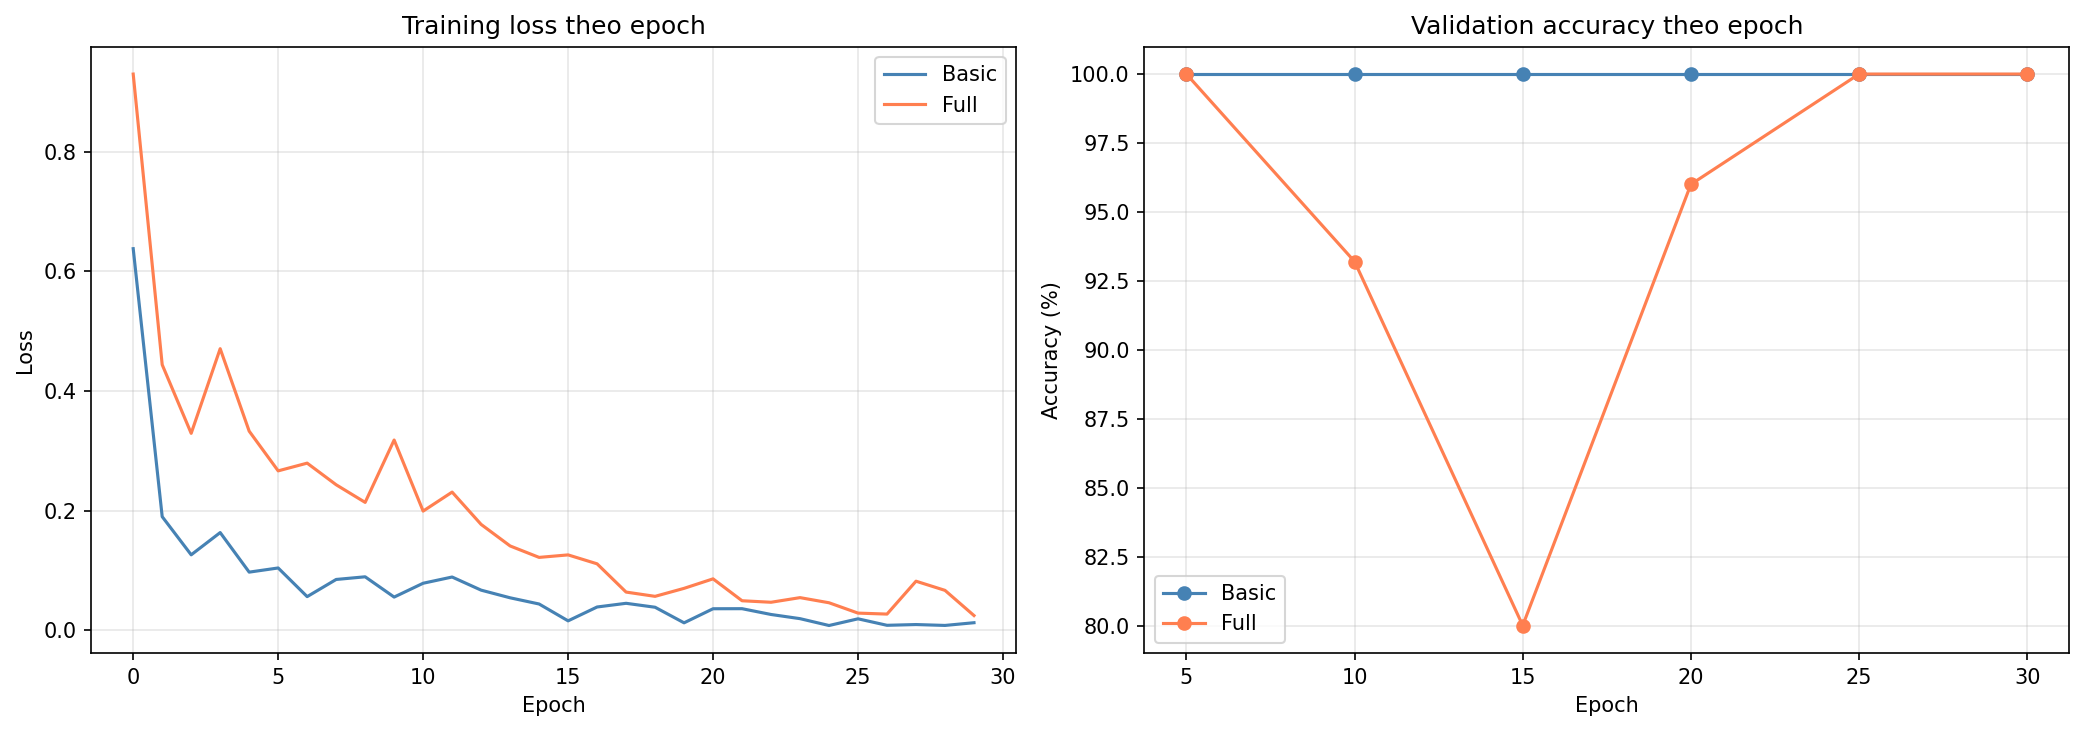
\includegraphics[width=0.82\textwidth]{graphics/training_curves_2.png}
\caption{Đường cong huấn luyện của hai biến thể PointNet trên tập 5 lớp.}
\label{fig:demo-pointnet-training-curves}
\end{figure}

\begin{table}[H]
\centering
\caption{Kết quả huấn luyện hai biến thể PointNet.}
\label{tab:demo-part2-results}
\small
\renewcommand{\arraystretch}{1.3} % Tăng lên 1.3 để các dòng có khoảng cách thoáng hơn
% Sử dụng tabularx với tổng chiều rộng \textwidth
% Cột X sẽ tự động tính toán độ rộng còn lại. >{\raggedright\arraybackslash} giúp căn trái cột này một cách tự nhiên.
\begin{tabularx}{\textwidth}{@{} l c c >{\raggedright\arraybackslash}X @{}}
\toprule
\rowcolor{gray!20}
\textbf{Mô hình} & \textbf{Số tham số} & \textbf{Best validation accuracy} & \textbf{Nhận xét} \\
\midrule
PointNetBasic & 810,629 & 100.0\% & Nhẹ hơn, hội tụ nhanh và ổn định trên tập nhỏ \\
PointNetFull  & 3,471,054 & 100.0\% & Nhiều tham số hơn, có T-Net, dao động lớn hơn ở giữa quá trình train \\
\bottomrule
\end{tabularx}
\end{table}

\begin{figure}[H]
\centering
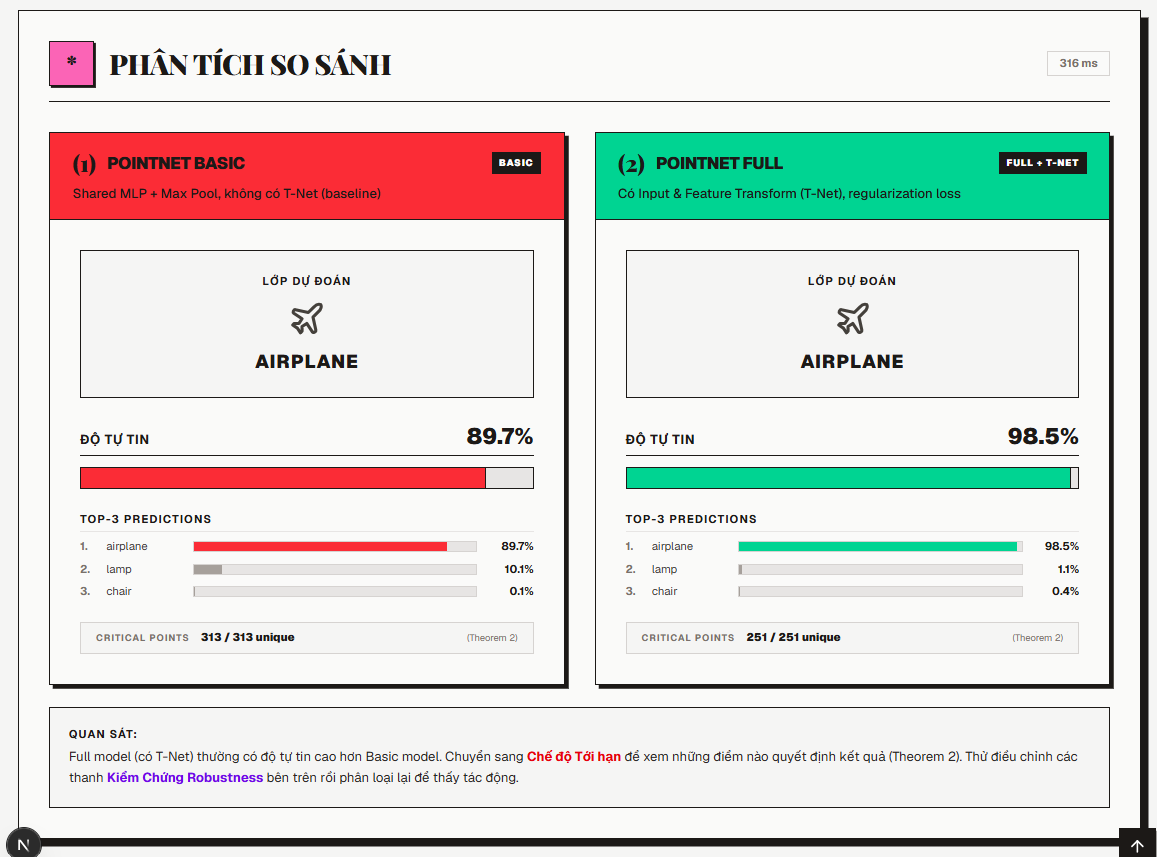
\includegraphics[width=0.90\textwidth]{graphics/result.png}
\caption{Kết quả phân loại trên giao diện demo cho vật thể máy bay.}
\label{fig:demo-part2-result}
\end{figure}

\noindent\textit{Ghi chú: PointNetBasic đạt 89.7\% độ tự tin, PointNetFull đạt 98.5\% trên cùng đầu vào. Top 3 dự đoán của cả hai mô hình được hiển thị cạnh nhau để dễ so sánh.}

Kết quả 100.0\% cần hiểu đúng trong phạm vi demo: chỉ có 5 lớp hình dạng khác biệt rõ, mục tiêu là minh họa chứ không phải benchmark. Con số này không nên hiểu là kết quả đại diện cho toàn bộ ModelNet40. Điều đáng chú ý hơn là demo giúp kiểm chứng tính bất biến hoán vị, cơ chế critical points và độ bền trước perturbation.

\subsubsection{Kiểm tra tính bất biến hoán vị}

Trong notebook, thứ tự điểm đầu vào được xáo trộn ngẫu nhiên 10 lần liên tiếp rồi so sánh logits của \texttt{PointNetFull}. Cả 10 lần đều cho cùng kết quả trong sai số tính toán. Điều này xác nhận tính bất biến hoán vị: thứ tự lưu điểm không ảnh hưởng đến dự đoán, vì kiến trúc chỉ dùng shared MLP và max pooling.

\begin{table}[H]
\centering
\caption{Kết quả kiểm tra tính bất biến hoán vị của PointNetFull.}
\label{tab:pointnet-permutation-test}
\small
\begin{tabular}{lc}
\toprule
\rowcolor{gray!20}
\textbf{Kiểm tra} & \textbf{Kết quả} \\
\midrule
Số lần shuffle thứ tự điểm & 10 \\
Logits giữ nguyên sau mỗi lần shuffle & True \\
Kết luận & Mô hình bất biến với hoán vị điểm \\
\bottomrule
\end{tabular}
\end{table}

\subsubsection{Robustness và critical points}

Demo hỗ trợ ba dạng perturbation: thay đổi số điểm đầu vào, thêm nhiễu Gaussian và bỏ ngẫu nhiên một tỉ lệ điểm. Các phép thử này giúp quan sát cách PointNet tóm tắt hình dạng. Do max pooling chỉ lấy giá trị lớn nhất ở mỗi kênh đặc trưng, chỉ một số ít điểm thực sự ảnh hưởng đến kết quả cuối, đó là critical points.

\begin{figure}[H]
\centering
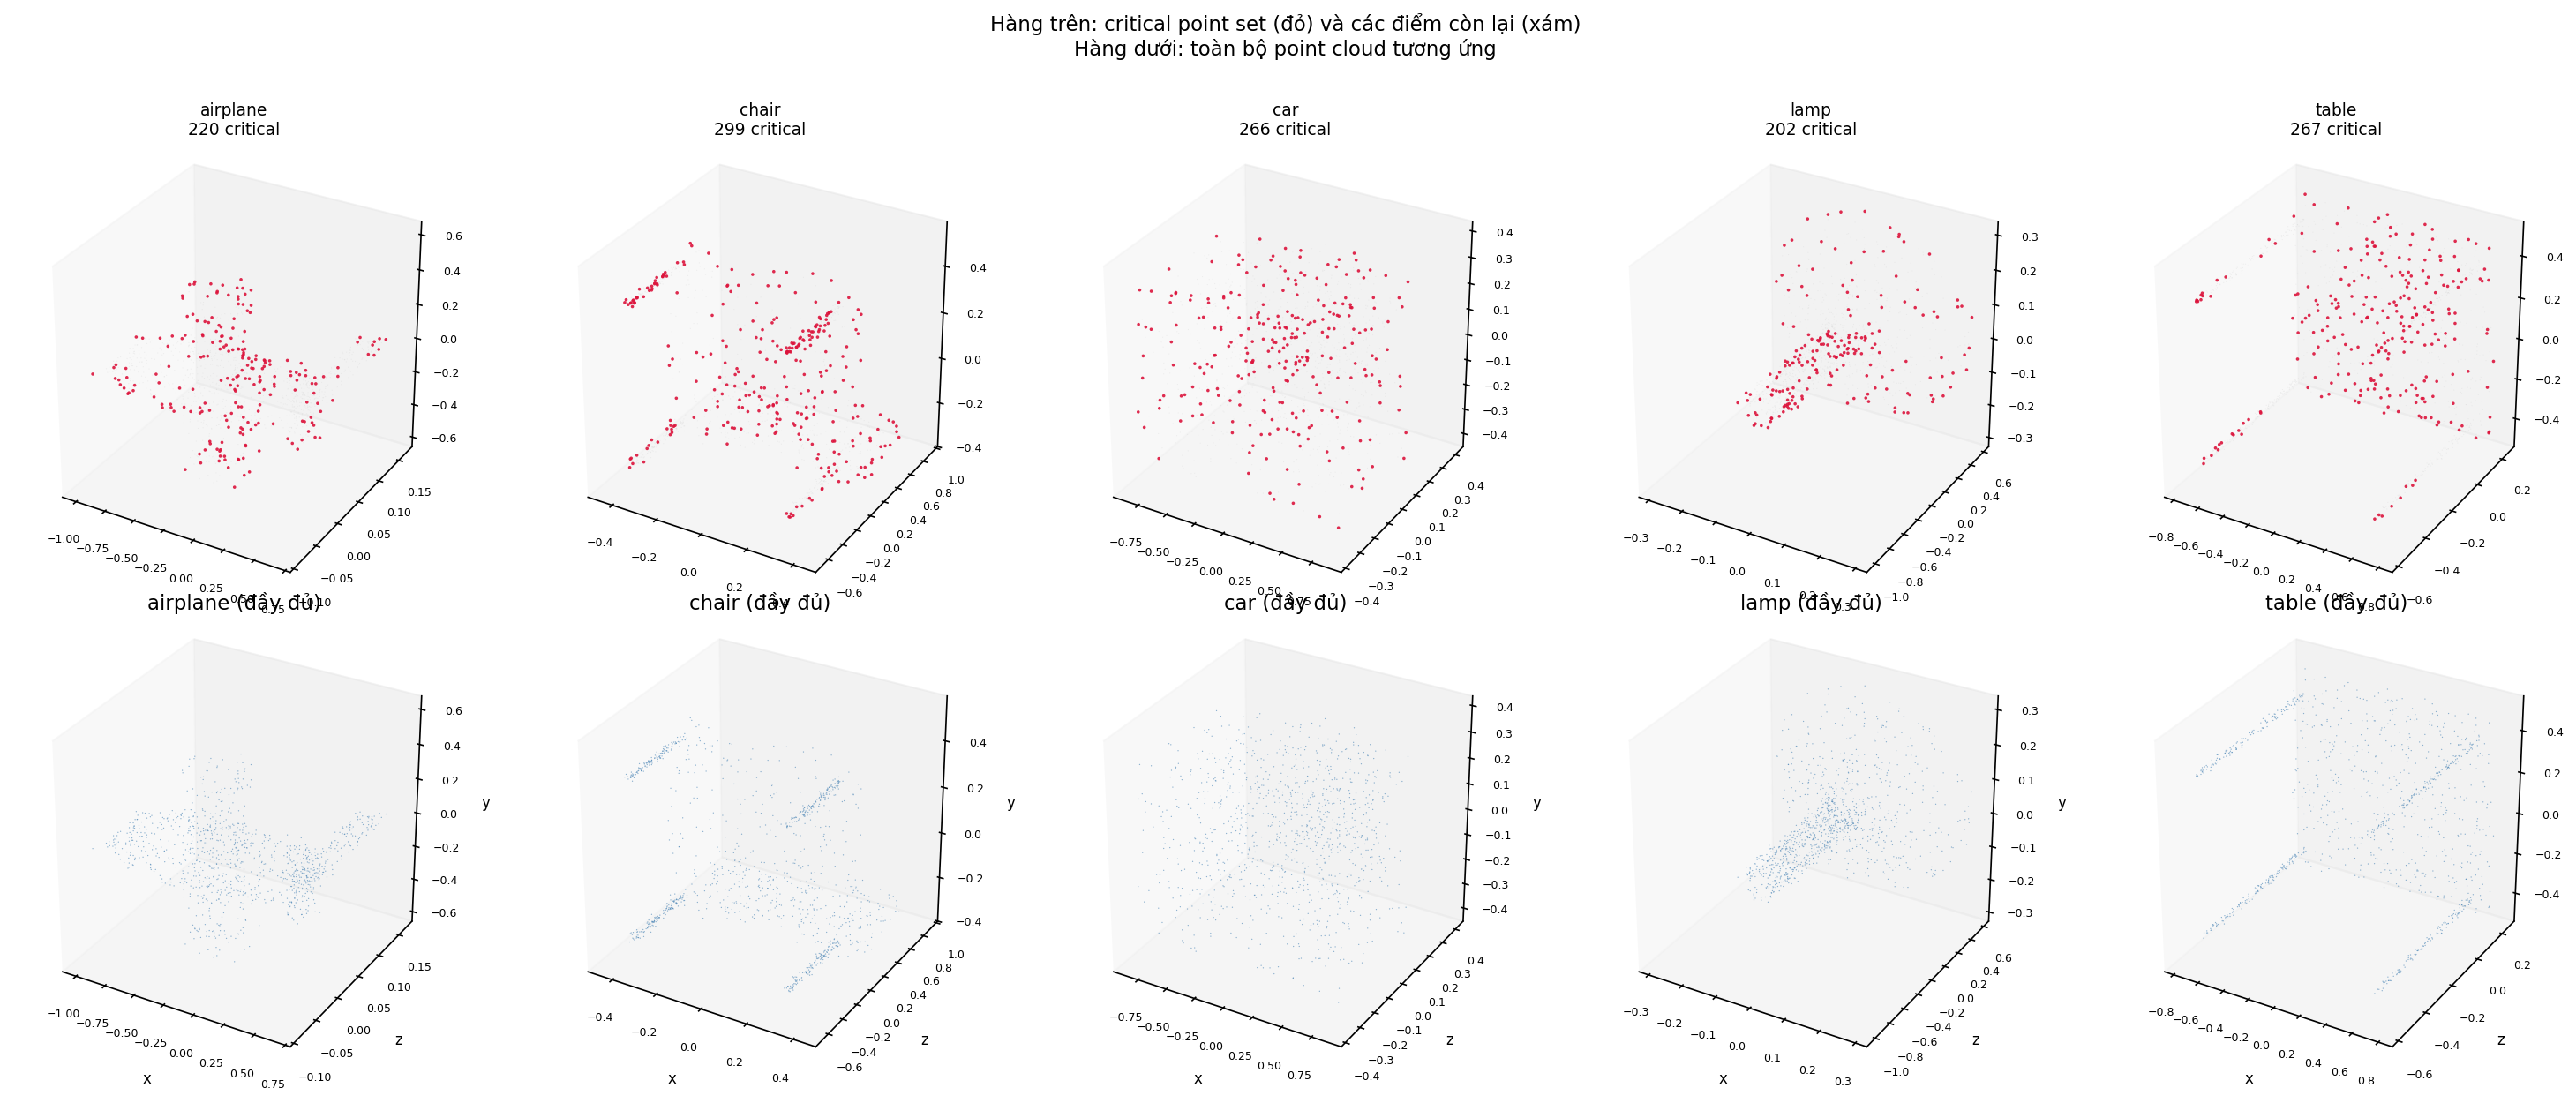
\includegraphics[width=0.90\textwidth]{graphics/critical_points_2.png}
\caption{Critical points của năm lớp vật thể.}
\label{fig:demo-critical-points}
\end{figure}

\noindent\textit{Ghi chú: Hàng trên là tập critical points màu đỏ, hàng dưới là toàn bộ point cloud màu xanh. Máy bay giữ lại khoảng 220 điểm tập trung ở cánh và thân, và ô tô giữ lại khoảng 266 điểm phân tán hơn do hình dạng ít đặc trưng hơn.}

\begin{figure}[H]
\centering
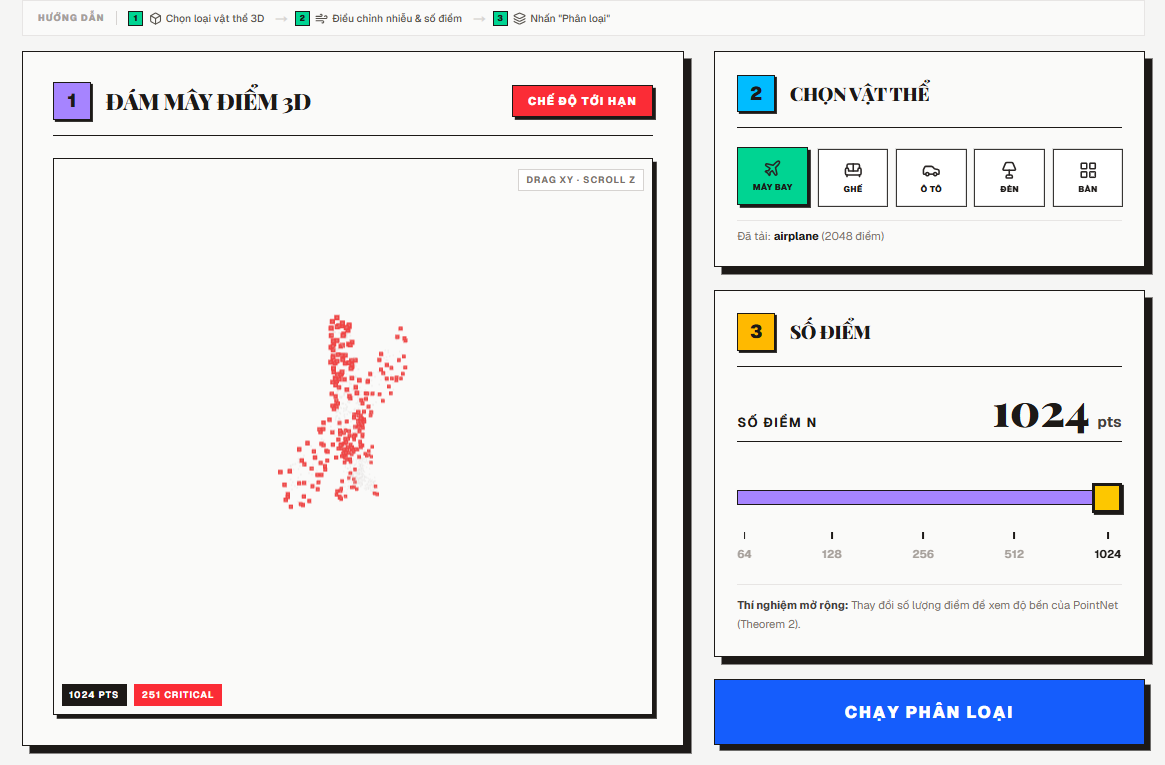
\includegraphics[width=0.7\textwidth]{graphics/flight-critical-point.png}
\caption{Các critical points được hiển thị trên mô hình máy bay trong chế độ trực quan hóa điểm tới hạn của hệ thống demo web.}
\label{fig:flight-critical-point}
\end{figure}

\begin{figure}[H]
\centering
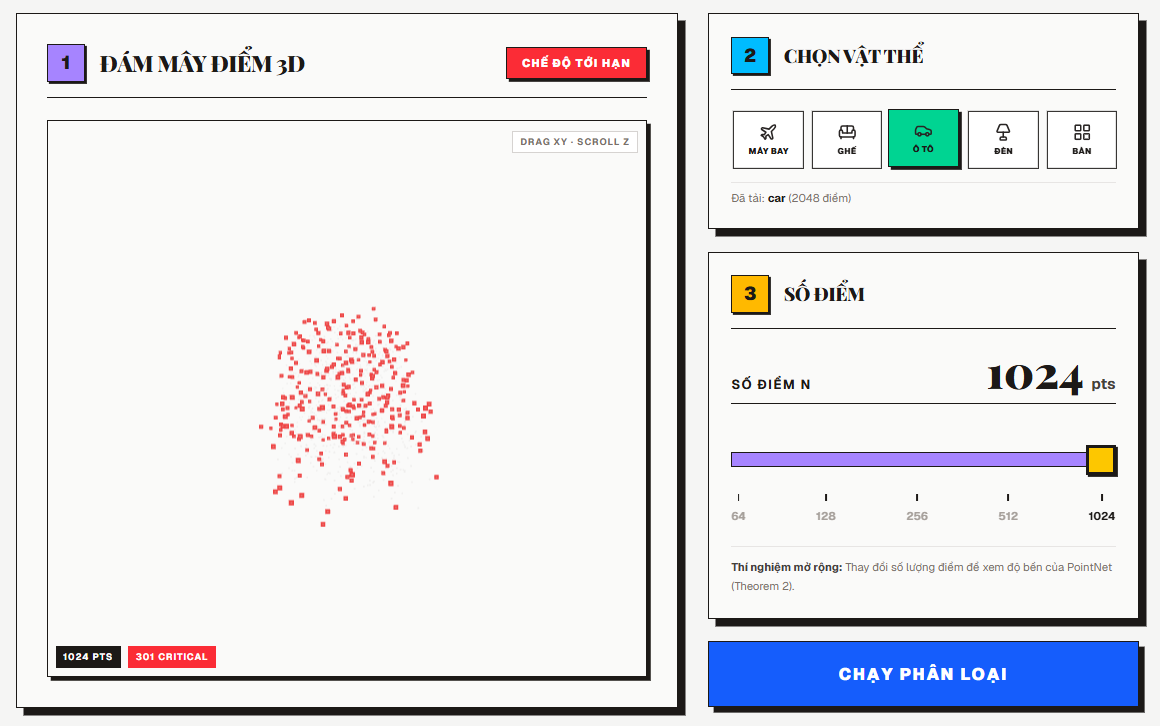
\includegraphics[width=0.7\textwidth]{graphics/oto-critical-point.png}
\caption{Các critical points được hiển thị trên mô hình ô tô trong chế độ trực quan hóa điểm tới hạn của hệ thống demo web.}
\label{fig:car-critical-point}
\end{figure}

\noindent\textit{Ghi chú: Máy bay (trái, 251 điểm) và ô tô (phải, 301 điểm). Các điểm màu đỏ là những điểm mà max pooling chọn ra ở ít nhất một kênh đặc trưng.}

Khi giảm số điểm hoặc bỏ ngẫu nhiên một phần, mô hình vẫn dự đoán đúng nếu các critical points quan trọng còn đó. Khi bỏ quá nhiều hoặc nhiễu Gaussian làm mờ các vùng biên, kết quả bắt đầu sai. Điều này khớp với phân tích ở Mục~\ref{sec:pointnet-paper}: PointNet không cần ghi nhớ toàn bộ bề mặt, chỉ cần một ít điểm đủ để phân biệt lớp là được.

\begin{figure}[H]
\centering
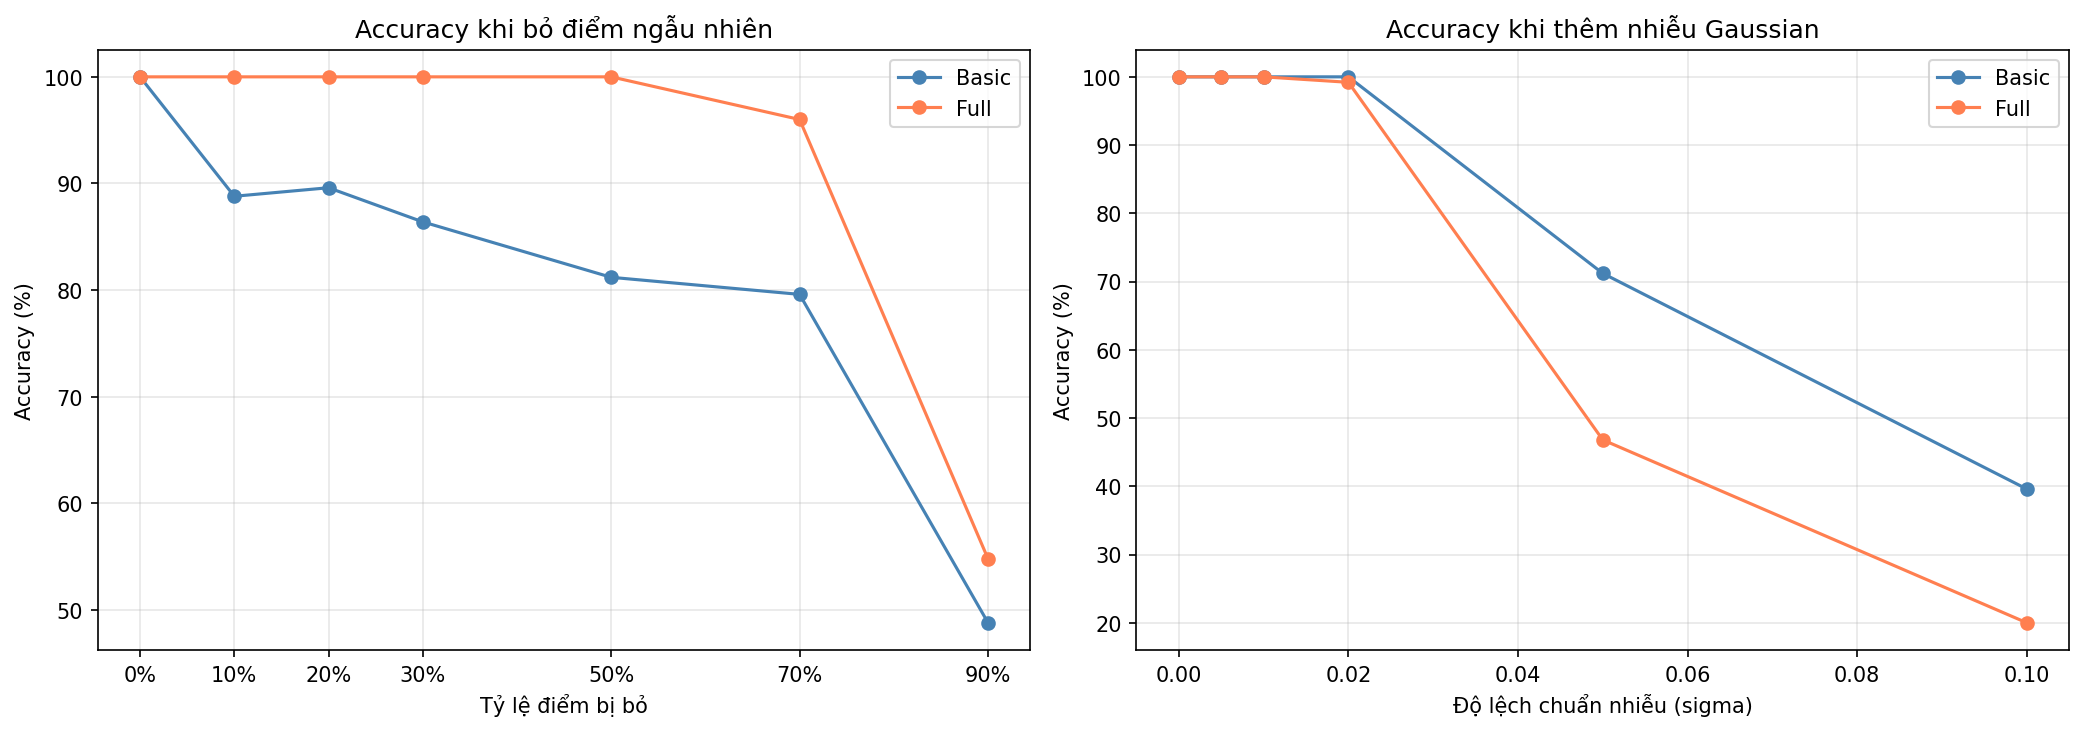
\includegraphics[width=0.90\textwidth]{graphics/robustness_2.png}
\caption{Accuracy của hai mô hình theo tỉ lệ điểm bị bỏ (trái) và theo mức nhiễu Gaussian (phải).}
\label{fig:demo-pointnet-robustness}
\end{figure}

\noindent\textit{Ghi chú: PointNetFull giữ accuracy cao hơn khi bỏ điểm ngẫu nhiên, trong khi PointNetBasic lại chịu nhiễu Gaussian tốt hơn ở mức cao.}

\begin{figure}[H]
\centering
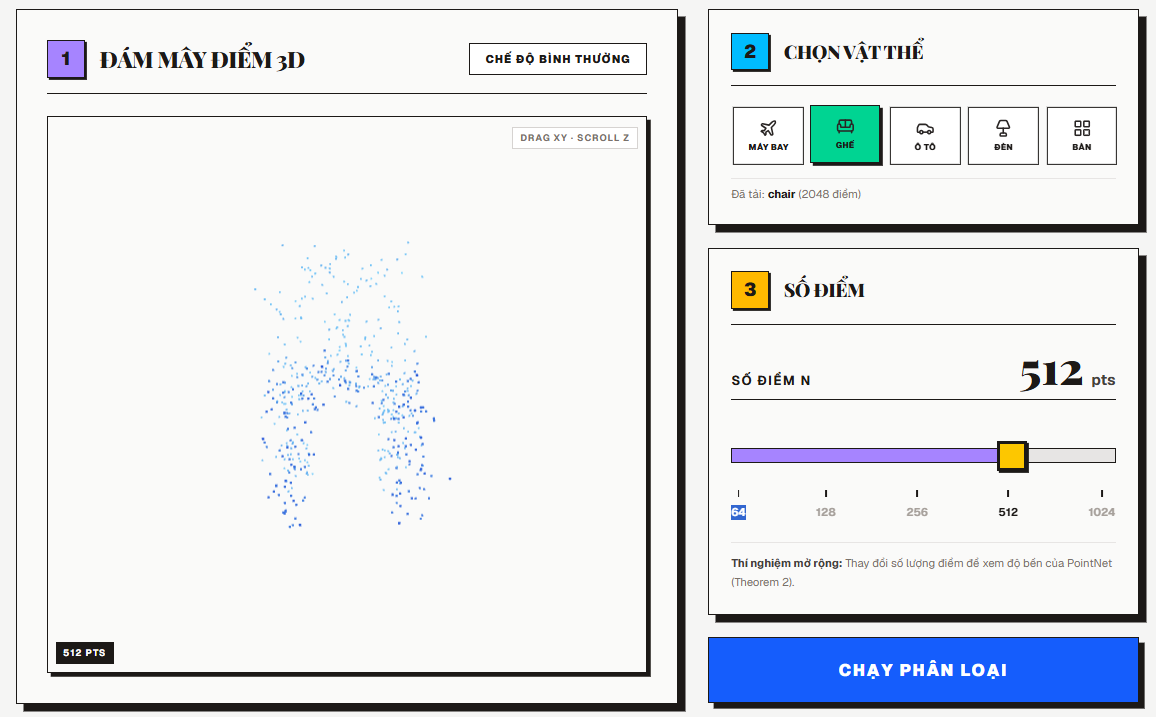
\includegraphics[width=0.6\textwidth]{graphics/ghe-512pts.png}
\caption{Mô hình ghế sau khi giảm mẫu còn 512 điểm, vẫn bảo toàn được hình dạng tổng thể của đối tượng.}
\label{fig:chair-512pts}
\end{figure}

\begin{figure}[H]
\centering
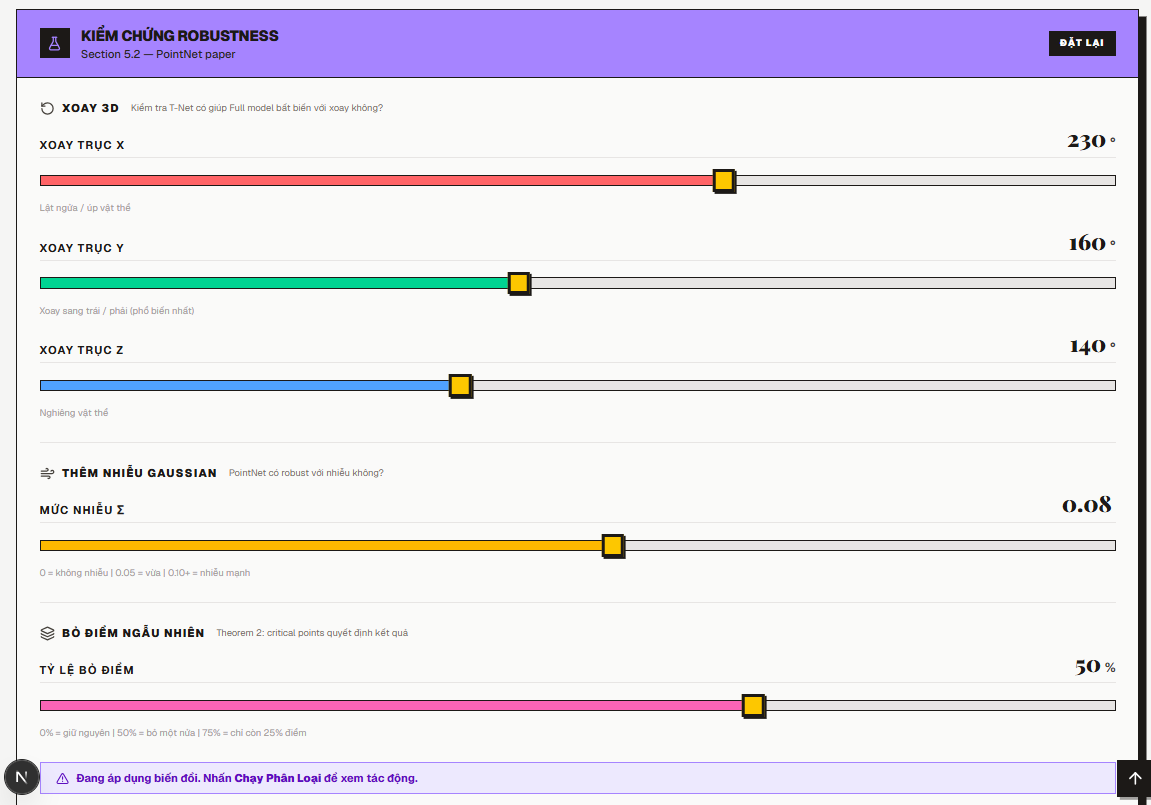
\includegraphics[width=0.8\textwidth]{graphics/dieu-chinh-flight.png}
\caption{Giao diện điều chỉnh perturbation trong hệ thống demo với các phép xoay độc lập theo trục X/Y/Z, thêm nhiễu Gaussian và loại bỏ ngẫu nhiên điểm.}
\label{fig:perturbation-panel}
\end{figure}

\subsection{Demo thực nghiệm Part 3: Dự đoán năng lượng phân tử với NequIP}
\label{subsec:demo-part3}

Demo thứ ba minh họa bài toán dự đoán nội năng $U_0$ của một phân tử cô lập bằng mạng nơ-ron đồ thị đẳng biến $E(3)$. Người dùng chọn một trong bảy phân tử mẫu hoặc tự chỉnh sửa tọa độ nguyên tử trong bảng editor, sau đó nhấn nút dự đoán để nhận về giá trị $U_0$ (eV) cùng thời gian inference. Backend xây dựng đồ thị phân tử, chạy NequIP và trả về kết quả qua REST API.


\begin{figure}[H]
\centering
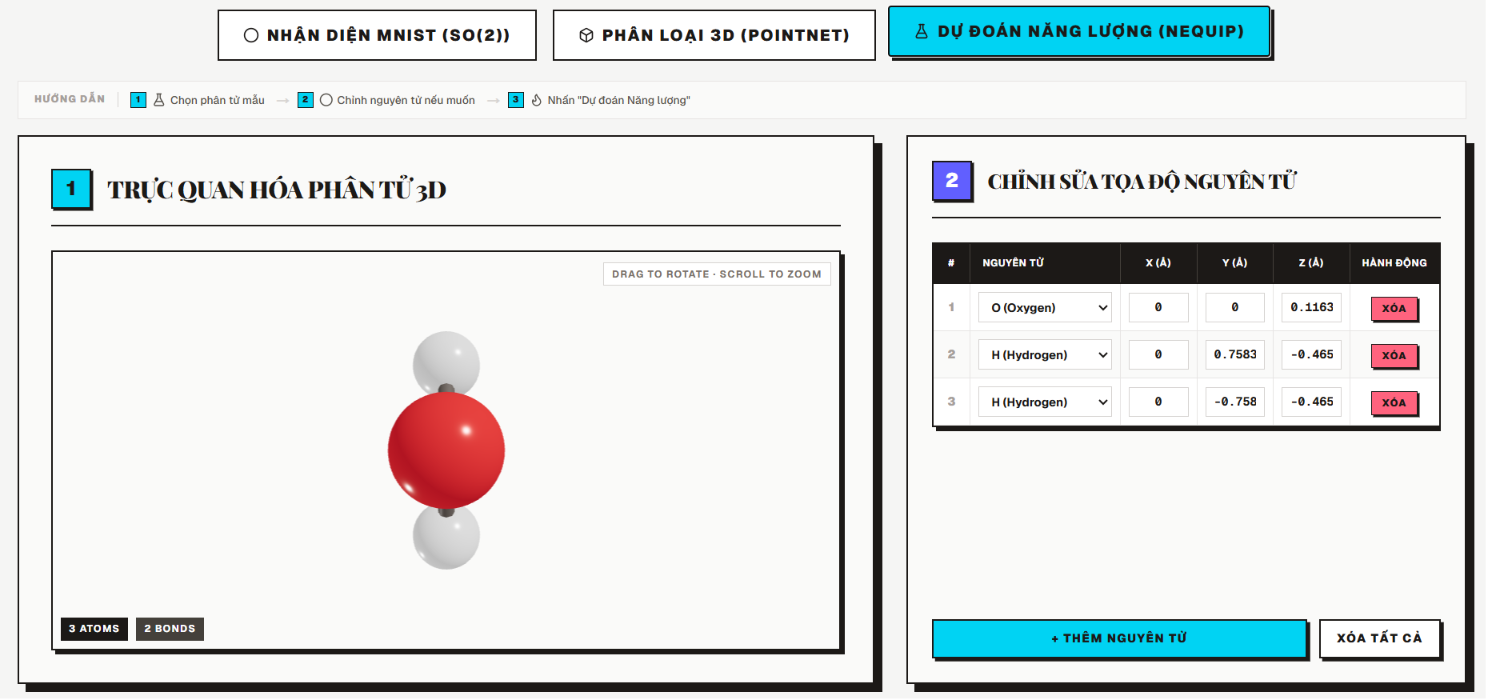
\includegraphics[width=0.95\textwidth]{graphics/demo_31.png}
\caption{Giao diện chính của demo Part 3 với mô hình phân tử 3D và bảng chỉnh sửa tọa độ nguyên tử.}
\label{fig:demo-part3-ui-editor}
\vspace{2mm}

\centering\textit{Ghi chú: Người dùng có thể quan sát cấu trúc phân tử ở khung 3D bên trái và thay đổi loại nguyên tử hoặc tọa độ $(x,y,z)$ ở bảng bên phải trước khi chạy dự đoán.}
\end{figure}

\begin{figure}[H]
\centering
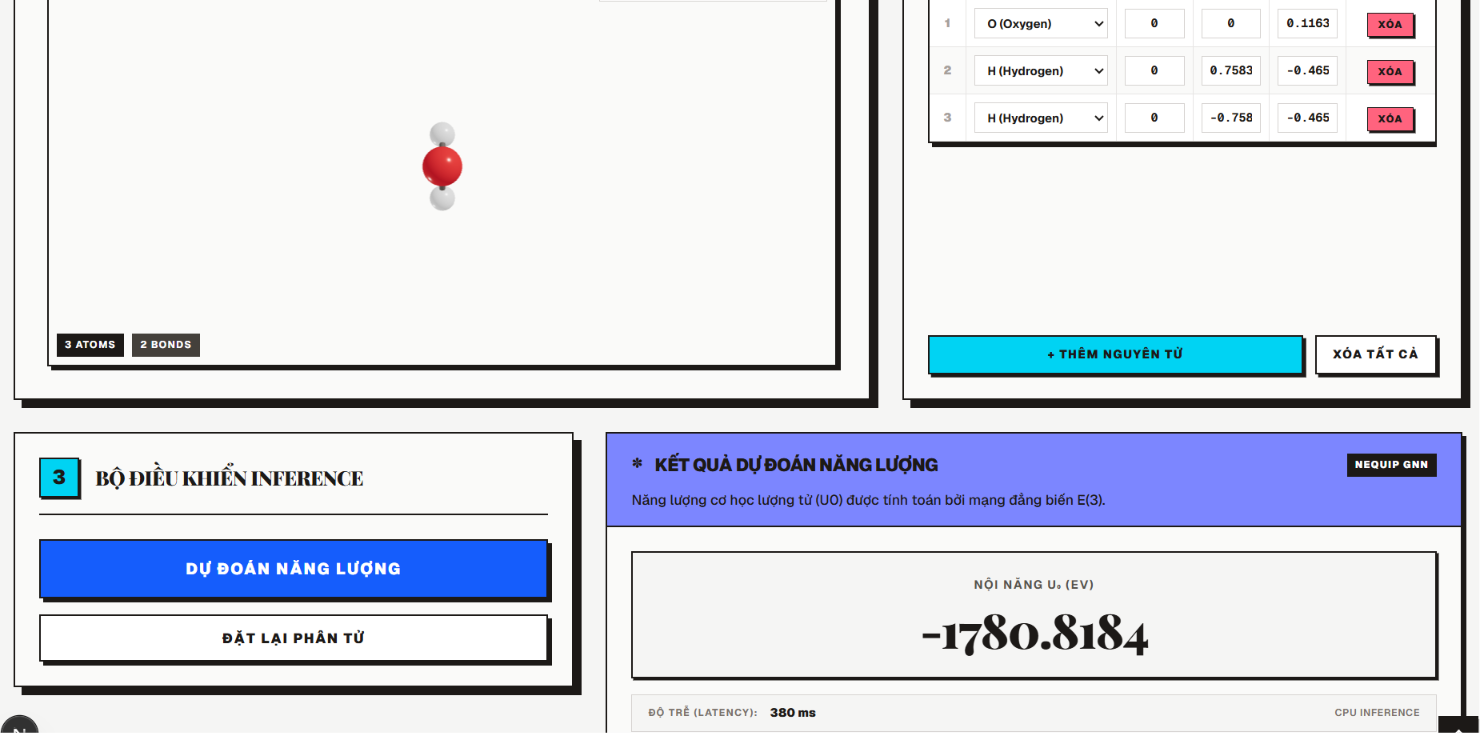
\includegraphics[width=0.95\textwidth]{graphics/demo_32.png}
\caption{Kết quả dự đoán nội năng phân tử trong demo Part 3.}
\label{fig:demo-part3-energy-result}
\vspace{2mm}

\centering\textit{Ghi chú: Sau khi nhấn nút dự đoán, backend chạy checkpoint NequIP và trả về nội năng $U_0$ theo đơn vị eV cùng độ trễ inference.}
\end{figure}

\begin{figure}[H]
\centering
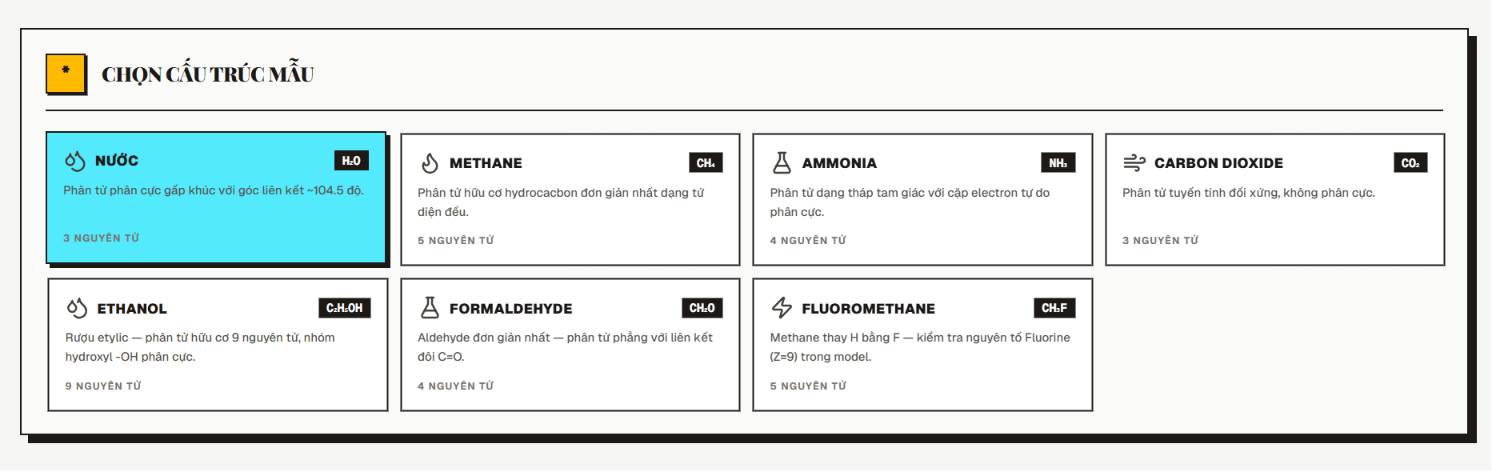
\includegraphics[width=0.95\textwidth]{graphics/demo_33.png}
\caption{Danh sách các cấu trúc phân tử mẫu trong demo Part 3.}
\label{fig:demo-part3-sample-selector}
\vspace{2mm}

\centering\textit{Ghi chú: Giao diện cung cấp bảy phân tử mẫu như nước, methane, ammonia, carbon dioxide, ethanol, formaldehyde và fluoromethane để người dùng thử nhanh mô hình.}
\end{figure}

\subsubsection{Bài toán và tính bất biến E(3)}

Nội năng $U_0$ là đại lượng vô hướng bất biến với mọi phép biến đổi thuộc nhóm $E(3)$: xoay, phản chiếu và tịnh tiến không làm thay đổi giá trị này. NequIP đảm bảo tính bất biến đó không phải bằng cách học từ dữ liệu, mà bằng cách xây dựng các đặc trưng ẩn \textit{đẳng biến} theo biểu diễn nhóm tương ứng. Khi tổng gộp toàn cục thu gọn các đặc trưng đẳng biến thành một đại lượng vô hướng, tính bất biến $E(3)$ của đầu ra được đảm bảo tự động từ cấu trúc kiến trúc mà không cần học từ dữ liệu.

\subsubsection{Dữ liệu và thiết lập thực nghiệm}

Demo huấn luyện trên tập con của QM9, tập dữ liệu hóa học lượng tử gồm khoảng 134.000 phân tử hữu cơ nhỏ với tối đa 9 nguyên tử nặng (C, N, O, F), tạo thành từ năm nguyên tố H, C, N, O, F. Nhãn $U_0$ của mỗi phân tử được tính bằng lý thuyết phiến hàm mật độ (DFT). Để quan sát hiệu quả dữ liệu, đồ án tạo hai tập con: 100 phân tử và 1000 phân tử. Các tập được chia theo tỉ lệ 80/10/10 (train/validation/test) và được dùng cho checkpoint triển khai trong demo.

\begin{figure}[H]
\centering

\includegraphics[width=0.80\textwidth]{graphics/qm9_molecules_3d.png}
\caption[Bảy phân tử mẫu cài sẵn trong demo Part 3]{Bảy phân tử mẫu cài sẵn trong giao diện demo Part 3.}
\label{fig:demo-part3-molecules}
\vspace{0.15cm}
\begin{minipage}{0.9\linewidth}
    \centering
\end{minipage}
\end{figure}

\vspace{-2.0em}
\noindent\textit{Ghi chú: Bảy cấu trúc gồm $\text{H}_2\text{O}$, $\text{CH}_4$, $\text{NH}_3$, $\text{CO}_2$, $\text{C}_2\text{H}_5\text{OH}$, $\text{CH}_2\text{O}$ và $\text{CH}_3\text{F}$. Fluoromethane là trường hợp thử nghiệm đặc biệt: nếu checkpoint không hỗ trợ nguyên tố F, backend trả về lỗi 422 kèm thông báo rõ ràng thay vì crash server.}

\subsubsection{Kiến trúc NequIP}

NequIP biểu diễn mỗi nguyên tử như một nút trong đồ thị; hai nút $i$ và $j$ được nối bằng cạnh khi khoảng cách $\|\vec{r}_{ij}\| < r_{\max} = 5{,}0\;\text{\AA}$. Đặc trưng cạnh kết hợp phần hướng kính (8 hàm Bessel với hàm cắt đa thức bậc $p = 6$) và phần góc (hàm điều hòa cầu $Y_\ell^m(\hat{r}_{ij})$ đến bậc $\ell_{\max}$). Quá trình message passing qua 4 tầng tương tác dùng tích Clebsch-Gordan để duy trì tính đẳng biến của các irreducible representation xuyên suốt. Sau 4 tầng, từ thành phần vô hướng ($\ell=0$) của mỗi nút, mạng đọc ra một năng lượng nguyên tử riêng; tổng các năng lượng nguyên tử này trên toàn đồ thị cho ra $U_0$.

\begingroup
\small
\renewcommand{\arraystretch}{1.25}
\setlength{\LTpre}{0.7\baselineskip}
\setlength{\LTpost}{0.9\baselineskip}
\begin{longtable}{@{}p{3.2cm} p{7.4cm} p{3.5cm}@{}}
\caption{Siêu tham số của mô hình NequIP triển khai trong demo Part 3.}
\label{tab:demo-part3-arch}\\
\toprule
\rowcolor{gray!20}
\textbf{Siêu tham số} & \textbf{Ý nghĩa} & \textbf{Giá trị} \\
\midrule
\endfirsthead
\toprule
\rowcolor{gray!20}
\textbf{Siêu tham số} & \textbf{Ý nghĩa} & \textbf{Giá trị} \\
\midrule
\endhead
Nguyên tố được hỗ trợ & Tập nguyên tử mô hình nhận được, trùng với 5 nguyên tố trong QM9 & H, C, N, O, F \\
Bán kính cắt $r_{\max}$ & Khoảng cách tối đa để nối cạnh; chỉ các cặp nguyên tử gần hơn ngưỡng này mới tương tác trực tiếp & $5{,}0\;\text{\AA}$ \\
Số tầng tương tác & Số lớp message passing; càng nhiều tầng, thông tin lan truyền càng xa trên đồ thị & 4 \\
$\ell_{\max}$ (cấu hình đẳng biến) & Bậc irreps cao nhất; $\ell_{\max}=1$ cho phép dùng đặc trưng vector có hướng, không chỉ vô hướng & 1 \\
Parity & Cho phép cả irrep chẵn và lẻ, giúp xử lý đúng phép phản chiếu (phân biệt vector và giả vector) & true (cả irrep chẵn và lẻ) \\
Số kênh đặc trưng & Độ rộng vector đặc trưng ẩn ở mỗi nút, quyết định dung lượng biểu diễn của mô hình & 32 \\
Hàm Bessel / bậc cắt $p$ & 8 hàm Bessel mã hóa khoảng cách thành biểu diễn liên tục; envelope đa thức bậc 6 làm đặc trưng cạnh tắt mượt về 0 tại $r_{\max}$ & 8 / 6 \\
Radial MLP & Mạng sinh trọng số phụ thuộc khoảng cách cho tích tensor, điều khiển cường độ tương tác theo $r$ & 2 tầng ẩn, 64 đơn vị \\
EMA decay & Trung bình động hàm mũ của trọng số, làm mượt và ổn định mô hình ở giai đoạn cuối & $0{,}999$ \\
Optimizer / learning rate & Thuật toán tối ưu adaptive với tốc độ học ban đầu & Adam / $5{\times}10^{-3}$ \\
LR scheduler & Giảm tốc độ học $\times 0{,}6$ khi val loss không cải thiện sau 10 epoch & ReduceLROnPlateau (factor $0{,}6$, patience 10) \\
Max epoch / early stopping & Huấn luyện tối đa 200 epoch, dừng sớm nếu val MAE không cải thiện sau 30 epoch & 200 / patience 30 \\
\bottomrule
\end{longtable}
\endgroup
\subsubsection{Luồng inference trong demo}

Khi người dùng nhấn nút dự đoán, frontend gửi danh sách \texttt{(atomic\_numbers, positions)} đến endpoint \texttt{/api/part3/predict-energy}. Backend thực hiện tuần tự: (1) xây dựng đối tượng \texttt{ASE Atoms} không tuần hoàn, (2) áp dụng \texttt{ChemicalSpeciesToAtomTypeMapper} để ánh xạ số nguyên tử sang chỉ số loại trong mô hình, (3) xây dựng danh sách lân cận trong bán kính $r_{\max}$ bằng \texttt{NeighborListTransform}, (4) chạy forward pass qua NequIP và trả về $U_0$ (eV). Toàn bộ pipeline chạy trên CPU với thời gian inference dưới 200 ms cho phân tử có ít hơn 10 nguyên tử.

\begin{figure}[H]
\centering
\resizebox{\textwidth}{!}{%
\begin{tikzpicture}[
  box/.style={rectangle, rounded corners=3pt, draw=black!40, line width=0.4pt,
              minimum width=1.9cm, minimum height=1.3cm, align=center,
              text=white, font=\scriptsize\bfseries},
  arr/.style={-{Stealth[length=2mm]}, line width=0.6pt, draw=black!55},
  lbl/.style={font=\tiny, text=black!70, align=center}
]
\node[box, fill=blue!55]                              (edit) {Molecule\\Editor\\(Frontend)};
\node[box, fill=orange!75, right=1.7cm of edit]       (ase)  {ASE\\Atoms};
\node[box, fill=purple!50, right=2.0cm of ase]        (graph){Neighbor\\Graph\\($r<5{,}0$\,\AA)};
\node[box, fill=green!50!black!75, right=1.7cm of graph](gnn) {NequIP GNN\\4 layers, $\ell=1$\\E(3)-equivariant};
\node[box, fill=magenta!60, right=1.7cm of gnn]       (out)  {Energy $U_0$\\(eV)};

\draw[arr] (edit)  -- node[lbl, above]{$Z$, pos}                       (ase);
\draw[arr] (ase)   -- node[lbl, above]{SpeciesToType\\+ NeighborList}  (graph);
\draw[arr] (graph) -- node[lbl, above]{Equivariant\\message passing}   (gnn);
\draw[arr] (gnn)   -- node[lbl, above]{Global\\sum pool}               (out);
\end{tikzpicture}}
\caption{Luồng chuyển đổi từ dữ liệu người dùng nhập vào đến đầu ra năng lượng $U_0$.}
\label{fig:demo-part3-flow}
\end{figure}

\subsubsection{So sánh bất biến và đẳng biến: hiệu quả dữ liệu}

Hai cấu hình được so sánh trên hai kích thước tập dữ liệu. \textit{Baseline} ($\ell_{\max}=0$) chỉ dùng đặc trưng vô hướng, bất biến $E(3)$ theo thiết kế nhưng thiếu thông tin hướng trong các biểu diễn ẩn. \textit{NequIP} ($\ell_{\max}=1$) bổ sung đặc trưng vector, cho phép mạng học các tương tác có hướng như liên kết cộng hóa trị và hiệu ứng cảm ứng.

\begin{figure}[H]
\centering
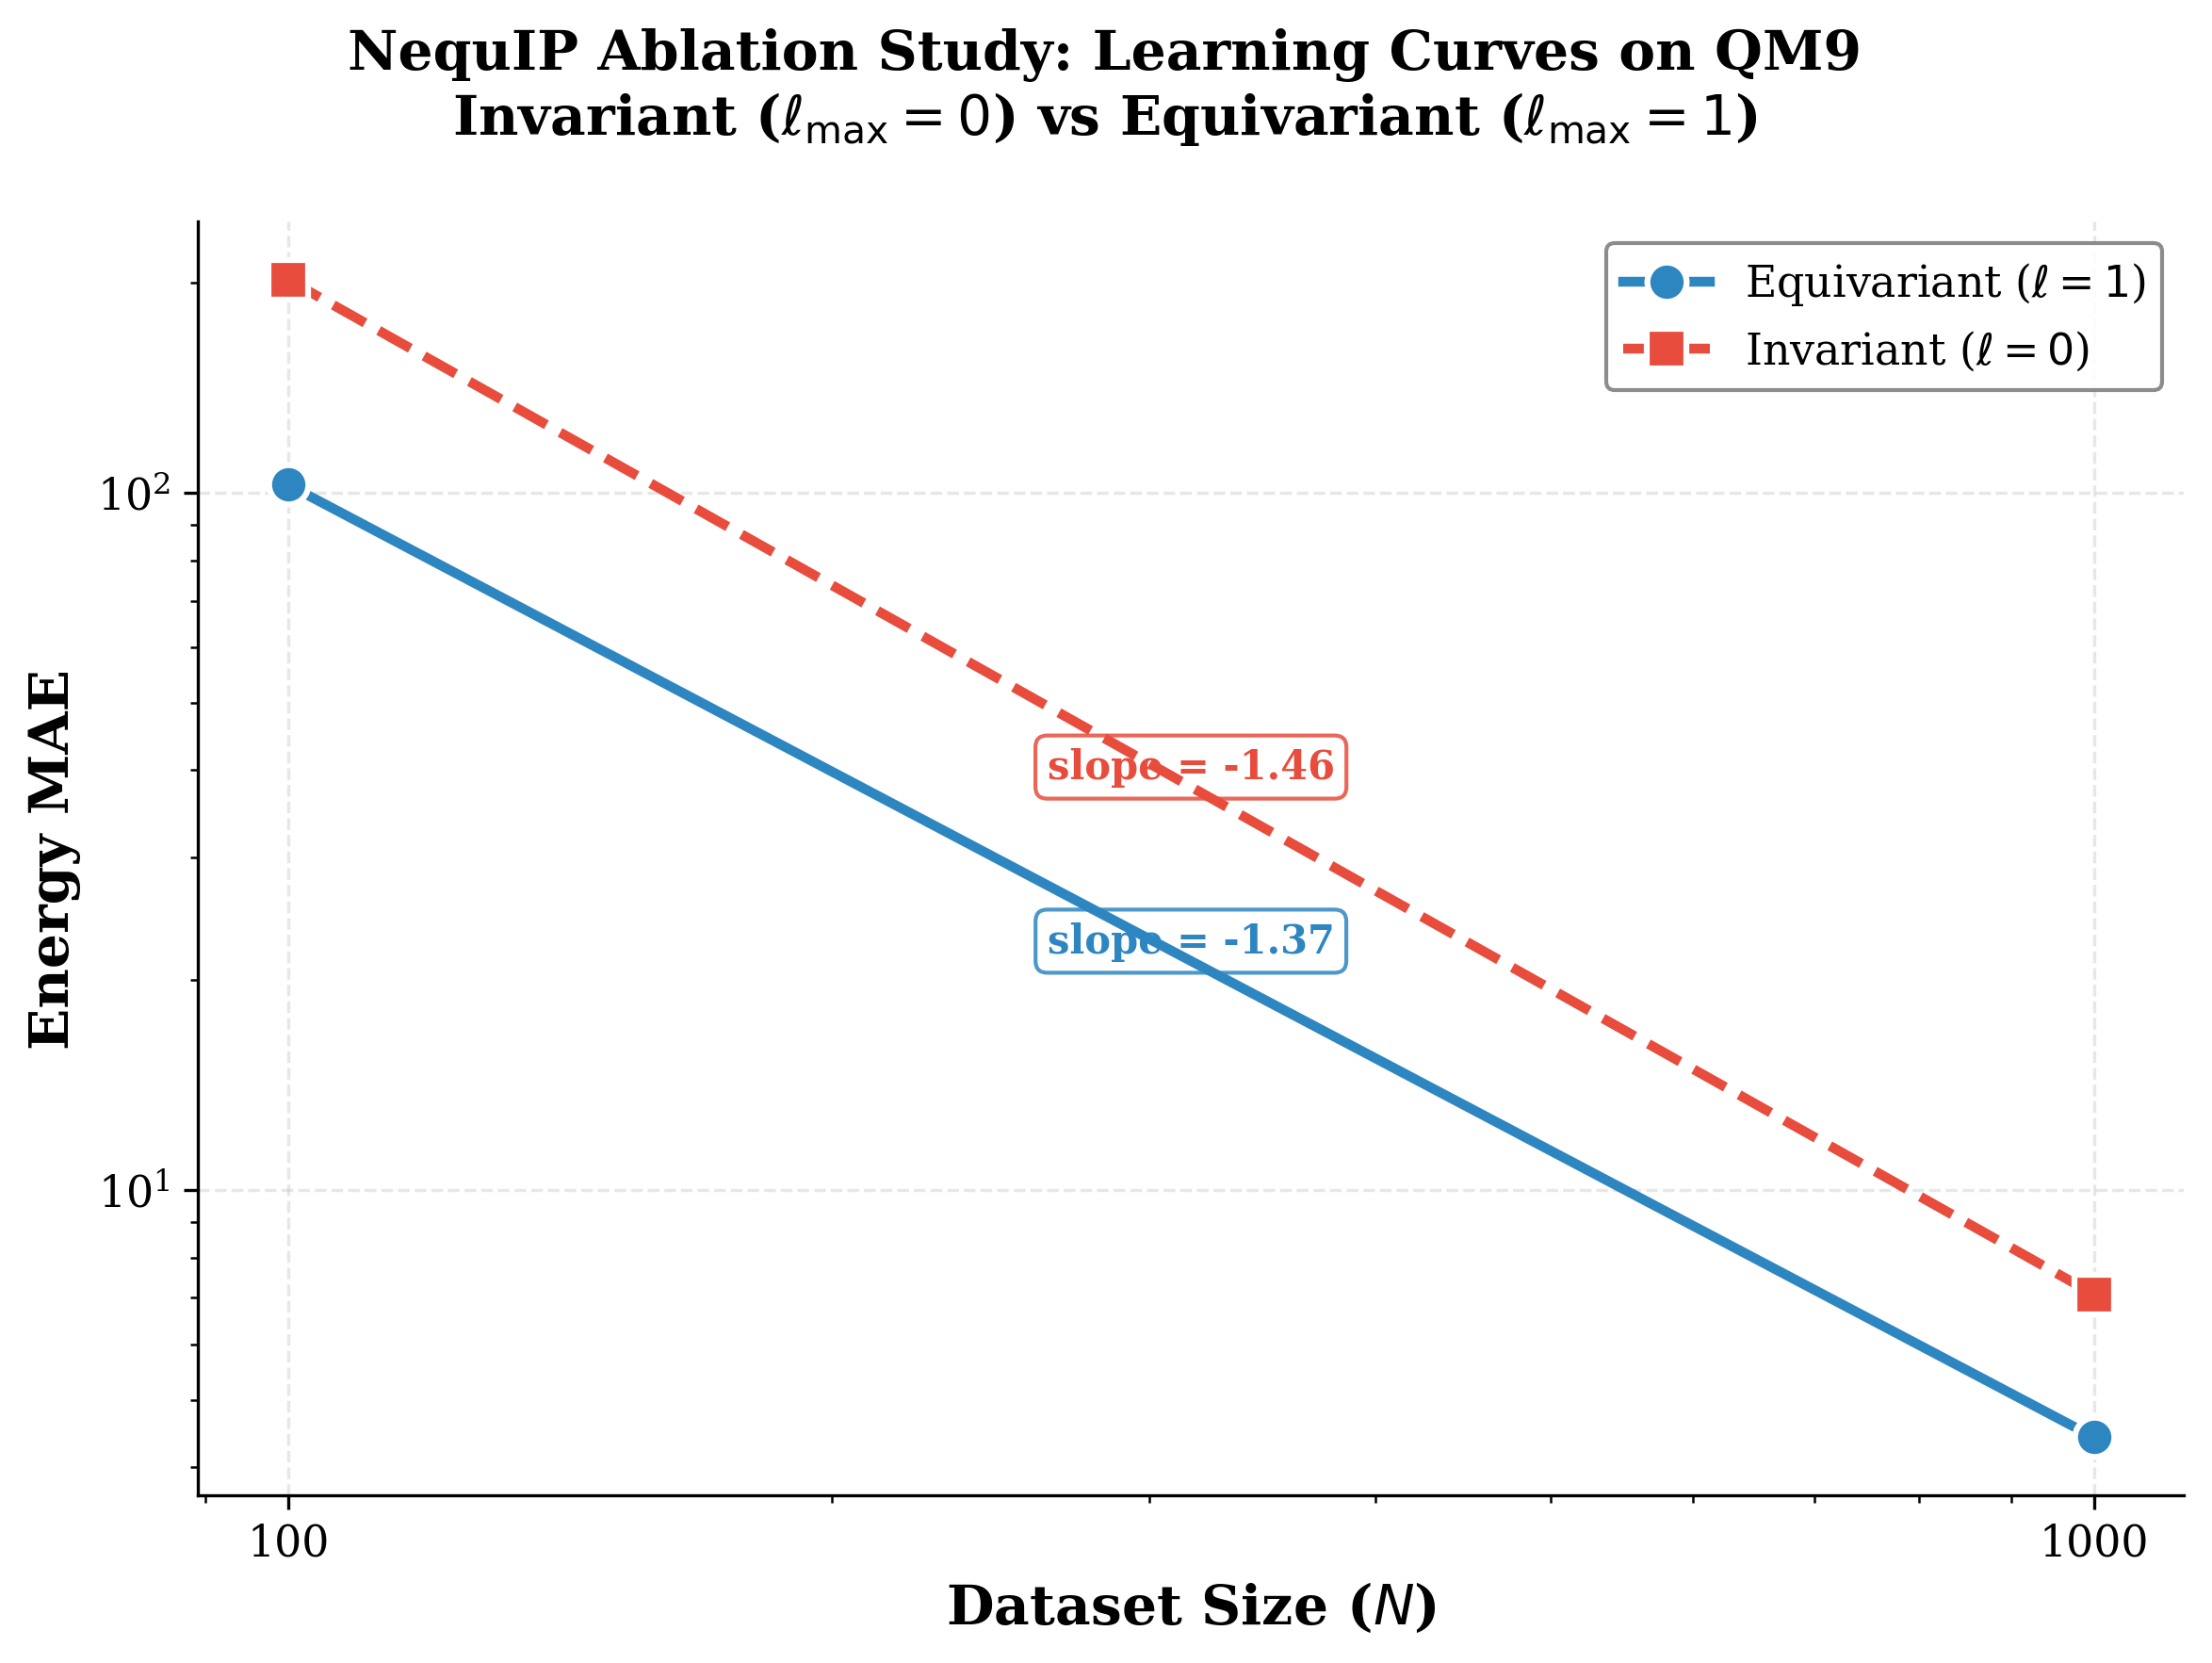
\includegraphics[width=0.65\textwidth]{graphics/nequip_learning_curve.png}
\caption[Đường học log-log của hai cấu hình NequIP trên QM9]{So sánh đường học của Baseline ($\ell_{\max}=0$) và NequIP ($\ell_{\max}=1$) trên hai kích thước tập dữ liệu.}
\label{fig:demo-part3-learning-curve}
\vspace{0.15cm}
\begin{minipage}{0.9\linewidth}
    \centering
\end{minipage}
\end{figure}

\vspace{-2.0em}
\noindent\textit{Ghi chú: Trục x là kích thước tập dữ liệu theo thang log; trục y là MAE năng lượng theo thang log.}

\begin{tcolorbox}[
  enhanced, breakable,
  colback=yellow!12!white,
  colframe=orange!85!black,
  coltitle=black,
  colbacktitle=yellow!55!orange,
  fonttitle=\bfseries,
  title=Nhận xét,
  boxrule=0.8pt, arc=2pt,
  left=2mm, right=2mm, top=1.5mm, bottom=1.5mm
]
\begin{itemize}[leftmargin=1.4em, itemsep=3pt, topsep=2pt]
  \item \textbf{Đẳng biến luôn tốt hơn:} Đường $\ell_{\max}=1$ nằm dưới đường $\ell_{\max}=0$ ở cả $N=100$ và $N=1000$, xác nhận lợi thế của việc mã hóa thông tin hướng qua hàm điều hòa cầu bậc~1.
  \item \textbf{Hiệu quả dữ liệu:} Khoảng cách giữa hai đường lớn hơn ở vùng $N$ nhỏ. Khi dữ liệu ít, việc cài sẵn đối xứng vật lý vào kiến trúc giúp mô hình đạt sai số thấp mà không cần nhiều mẫu huấn luyện.
  \item \textbf{Về độ dốc (slope log-log):} Mô hình bất biến dốc hơn ($-1{,}46$ so với $-1{,}37$), tức cải thiện theo dữ liệu nhanh hơn một chút; nhưng mô hình đẳng biến luôn xuất phát từ MAE thấp hơn nên vẫn tốt hơn ở mọi quy mô. Lợi thế chính của tính đẳng biến nằm ở mức sai số nền, không phải tốc độ scale.
  \item \textbf{Ý nghĩa thang log-log:} Đường thẳng trên trục log-log ứng với quan hệ lũy thừa $\text{MAE} \propto N^{\alpha}$, với $\alpha$ là slope; slope càng âm thì MAE giảm càng nhanh khi tăng dữ liệu.
\end{itemize}
\end{tcolorbox}

\begin{figure}[H]
\centering
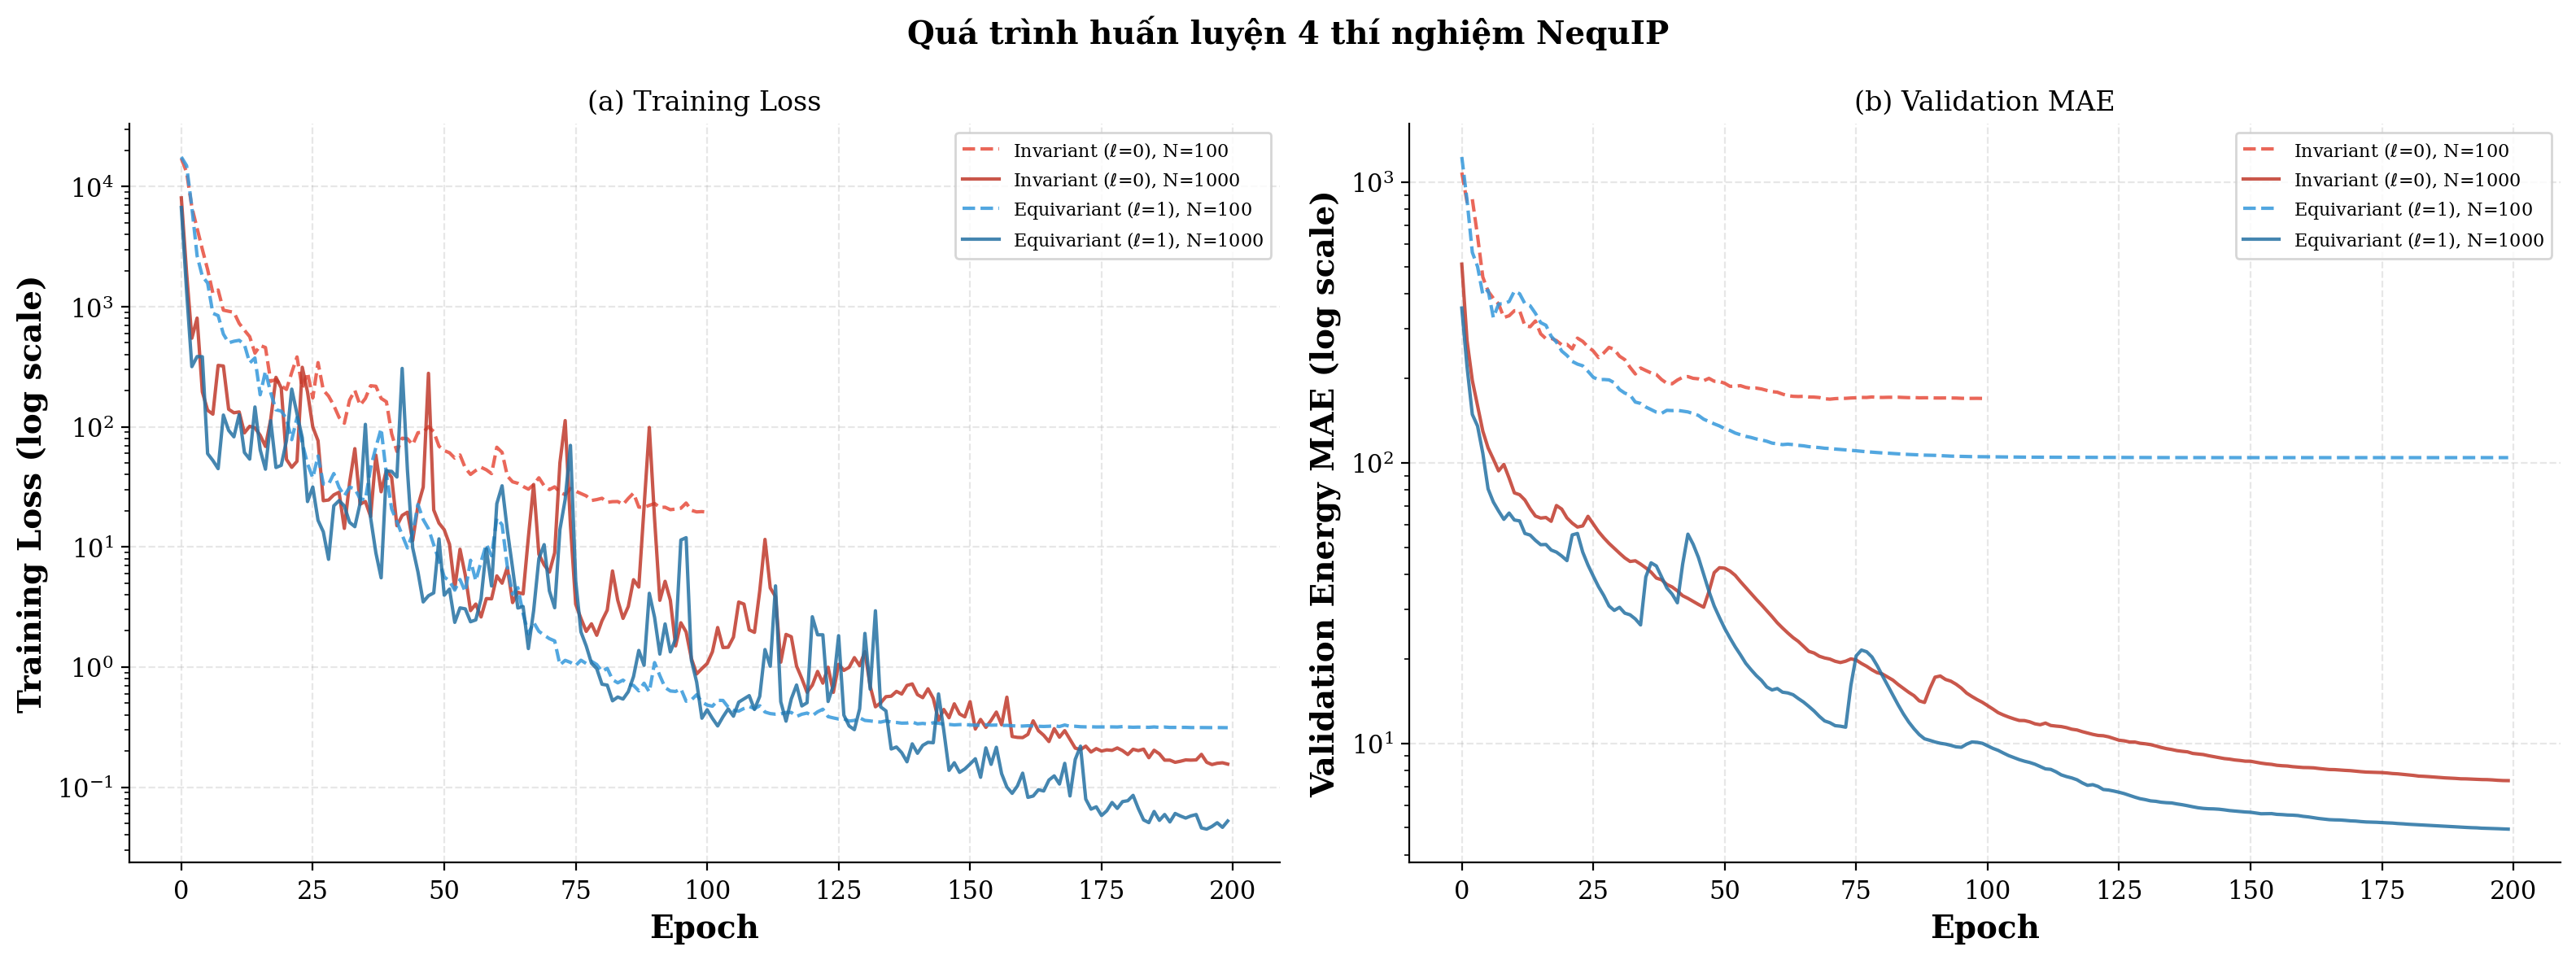
\includegraphics[width=0.95\textwidth]{graphics/nequip_training_curves.png}
\caption[Đường cong huấn luyện bốn thí nghiệm NequIP]{Đường cong training loss (a) và validation MAE (b) theo epoch cho bốn thí nghiệm: bất biến ($\ell_{\max}=0$) và đẳng biến ($\ell_{\max}=1$) trên hai kích thước tập dữ liệu $N=100$ và $N=1000$.}
\label{fig:demo-part3-training}
\end{figure}

\noindent\textit{Ghi chú: Early stopping kích hoạt khi validation MAE không cải thiện trong 30 epoch liên tiếp. EMA (ema\_decay $= 0{,}999$) ổn định quá trình tối ưu hóa ở giai đoạn cuối.}

\begin{tcolorbox}[
  enhanced, breakable,
  colback=blue!5!white,
  colframe=blue!55!black,
  coltitle=white,
  fonttitle=\bfseries,
  title=Nhận xét,
  boxrule=0.8pt, arc=2pt,
  left=2mm, right=2mm, top=1.5mm, bottom=1.5mm
]
\begin{itemize}[leftmargin=1.4em, itemsep=3pt, topsep=2pt]
  \item \textbf{(a) Training loss:} Cả bốn mô hình đều hội tụ. Ở cùng kích thước dữ liệu, loss của $\ell_{\max}=1$ giảm nhanh hơn $\ell_{\max}=0$ trong giai đoạn đầu, cho thấy tính đẳng biến giúp tối ưu hàm mất mát hiệu quả hơn.
  \item \textbf{(b) Validation MAE:} Trong khoảng epoch 0--50, mô hình $\ell_{\max}=1$ giảm MAE nhanh và rõ rệt hơn; sau khi hội tụ, khoảng cách giữa các mô hình thu hẹp lại.
  \item \textbf{Ảnh hưởng kích thước dữ liệu:} Các đường nét đứt ($N=100$, 10 phân tử validation) dao động mạnh hơn, trong khi nét liền ($N=1000$, 100 phân tử validation) mượt và ổn định hơn.
  \item \textbf{Cơ chế ổn định:} Mô hình $N=1000$ cần nhiều epoch hơn để ổn định do tập huấn luyện lớn hơn; early stopping (patience 30) và EMA ($0{,}999$) giúp tránh overfitting và làm mượt giai đoạn cuối.
\end{itemize}
\end{tcolorbox}

\subsection{Thảo luận chung và liên kết lý thuyết}
\label{subsec:thao-luan-thuc-nghiem}

\subsubsection{Tính bất biến xấp xỉ và tính bất biến do kiến trúc}

Ba demo cho thấy ba cách khác nhau để đưa inductive bias hình học vào mô hình. Trong Part 1, Augmented CNN học tính bất biến từ dữ liệu, nên tính bất biến chỉ là xấp xỉ và có thể thất bại ở các trường hợp nhãn mơ hồ. Frame Averaging CNN đưa cấu trúc frame vào bước suy luận, nhờ đó có cơ chế xử lý xoay rõ ràng hơn. Trong Part 2, tính bất biến với hoán vị không cần học từ dữ liệu: nó xuất hiện trực tiếp từ thiết kế shared MLP và max pooling. Trong Part 3, tính bất biến $E(3)$ của đầu ra được đảm bảo qua lý thuyết biểu diễn nhóm: các đặc trưng ẩn đẳng biến theo irreducible representation, và phép tổng gộp toàn cục tự động kết nạp tính bất biến mà không cần bất kỳ xử lý hậu kỳ nào.

\subsubsection{Hiệu quả dữ liệu và giới hạn của demo}

Các kết quả trong chương này cần được hiểu như minh họa thực nghiệm cho lý thuyết, không phải benchmark đầy đủ trên quy mô lớn. Part 1 dùng MNIST để làm rõ ảnh hưởng của phép xoay trong môi trường dễ quan sát. Part 2 dùng 5 lớp trích từ ModelNet40 để giao diện demo nhẹ và phản hồi nhanh. Part 3 dùng tập con 1000 phân tử của QM9 để minh họa lợi ích của đẳng biến $E(3)$ trên dữ liệu phân tử thực tế. Giá trị MAE trong Part 3 phản ánh tập huấn luyện nhỏ và không nên so sánh trực tiếp với các kết quả công bố trên toàn bộ QM9.

Dù vậy, xu hướng chung vẫn nhất quán với lý thuyết ở Chương~\ref{sec:phuong-phap}: khi cấu trúc đối xứng được đưa vào mô hình, mô hình cần ít dữ liệu hơn để học cùng một quy luật và có hành vi ổn định hơn trước các biến đổi không làm thay đổi bản chất đối tượng.

\subsubsection{Đối chiếu hai hướng tiếp cận}

\begin{table}[H]
\centering
\small
\renewcommand{\arraystretch}{1.3}
\caption{Đối chiếu ba demo thực nghiệm qua lăng kính ba hướng tiếp cận geometric machine learning.}
\label{tab:demo-lien-ket}
\begin{tabularx}{\textwidth}{p{0.17\textwidth}>{\raggedright\arraybackslash}X>{\raggedright\arraybackslash}X>{\raggedright\arraybackslash}X}
\toprule
\rowcolor{gray!20}
\textbf{Tiêu chí} & \textbf{Part 1: MNIST xoay} & \textbf{Part 2: PointNet} & \textbf{Part 3: NequIP} \\
\midrule
Đối tượng dữ liệu & Ảnh $28\times28$ trên lưới 2D & Tập điểm không có thứ tự trong không gian 3D & Phân tử hóa học với tọa độ nguyên tử 3D \\
Nhóm đối xứng & $SO(2)$, phép xoay liên tục & $S_n$, phép hoán vị hữu hạn & $E(3)$, nhóm Euclidean trong $\mathbb{R}^3$ \\
Cách đưa đối xứng vào mô hình & Data augmentation hoặc frame averaging & Shared MLP và max pooling & Equivariant message passing với irrep \\
Loại bất biến & Xấp xỉ với augmentation, rõ ràng hơn với frame averaging & Bất biến hoán vị ngay từ kiến trúc & Bất biến $E(3)$ được đảm bảo bằng biểu diễn nhóm \\
Giới hạn chính & Ambiguity nhãn khi xoay một số chữ số & Demo chỉ dùng 5 lớp, chưa đại diện toàn bộ ModelNet40 & Tập huấn luyện nhỏ (1000 phân tử), chưa tính lực \\
\bottomrule
\end{tabularx}
\end{table}

Từ ba demo, có thể rút ra kết luận rằng inductive bias hình học không chỉ giúp tăng độ chính xác trong một số thiết lập, mà quan trọng hơn là làm cho hành vi của mô hình nhất quán hơn với cấu trúc của dữ liệu. Với ảnh xoay, mô hình cần hiểu quan hệ giữa các góc. Với point cloud, mô hình cần bỏ qua thứ tự lưu trữ điểm. Với phân tử hóa học, mô hình cần đảm bảo rằng xoay hay phản chiếu toàn bộ phân tử không thay đổi năng lượng dự đoán. Ba yêu cầu này tương ứng với ba cơ chế khác nhau để tích hợp đối xứng vào học máy, và đây chính là vai trò trung tâm của geometric machine learning: thiết kế mô hình không chỉ dựa trên dữ liệu đầu vào, mà còn dựa trên những phép biến đổi mà bài toán cho phép hoặc cần bất biến theo.

\clearpage

\section*{Phụ lục: Phân công công việc nhóm}
\addcontentsline{toc}{section}{Phụ lục: Phân công công việc nhóm}

\newlist{tableitemize}{itemize}{1}
\setlist[tableitemize]{
    label=\textbullet,
    leftmargin=1.1em,
    nosep,
    topsep=0pt,
    partopsep=0pt,
    parsep=0pt,
    itemsep=2pt,
    before=\vspace{-0.4\baselineskip},
    after=\vspace{0.1\baselineskip}
}

\begingroup
\small
\renewcommand{\arraystretch}{1.2}
\newcounter{memberrow}
\setcounter{memberrow}{0}

\begin{longtable}{|>{\stepcounter{memberrow}\thememberrow}c|p{3.2cm}|c|p{9.5cm}|}
\hline
\rowcolor[HTML]{E8E8E8}
\multicolumn{1}{|c|}{\textbf{STT}} & \centering\textbf{Họ và tên} & \textbf{MSSV} & \centering\arraybackslash\textbf{Nhiệm vụ chính} \\
\hline
\endfirsthead

\hline
\rowcolor[HTML]{E8E8E8}
\multicolumn{1}{|c|}{\textbf{STT}} & \centering\textbf{Họ và tên} & \textbf{MSSV} & \centering\arraybackslash\textbf{Nhiệm vụ chính (tiếp theo)} \\
\hline
\endhead

\textbf{} & \textbf{Lê Hà Thanh Chương} & 23120195 &
\begin{tableitemize}
    \item \textbf{Quản lý dự án \& Tổng hợp:} Quản lý tiến độ tổng thể, thiết lập môi trường latex; chuẩn hóa định dạng, mục lục, danh mục thuật ngữ và ráp nối toàn bộ báo cáo.
    \item \textbf{Nghiên cứu \& Báo cáo:} Phụ trách Chương 1 (Giới thiệu, bối cảnh và động lực) và Chương 5 (Thực nghiệm chi tiết, đặc biệt nghiên cứu sâu kiến trúc NequIP).
    \item \textbf{Thực nghiệm \& Ứng dụng:} Trực tiếp xây dựng hệ thống Demo Web toàn bộ Part 3 (NequIP, QM9) để trực quan hóa năng lực dự đoán cấu trúc phân tử.
\end{tableitemize} \\ \hline

\textbf{} & \textbf{Trà Văn Sỹ} & 23120197 &
\begin{tableitemize}
    \item \textbf{Nghiên cứu \& Báo cáo:} Phụ trách Mục 3.1 và 3.2 của Chương 3 (Các phương pháp xây dựng mô hình bảo toàn đối xứng cơ bản) và Chương 6 (Đánh giá tổng thể \& Kết luận).
    \item \textbf{Thực nghiệm \& Kỹ thuật:} Khởi tạo và thiết lập nền tảng Web Frontend ban đầu cho dự án. Xây dựng mã nguồn Demo Part 1 (MNIST xoay, CNN Tương biến) và soạn thảo Jupyter Notebook minh họa.
\end{tableitemize} \\ \hline

\textbf{} & \textbf{Huỳnh Đức Thịnh} & 23120199 &
\begin{tableitemize}
    \item \textbf{Nghiên cứu \& Báo cáo:} Phụ trách các phần còn lại của Chương 3 (tập trung phân tích chuyên sâu kiến trúc mạng PointNet và các cơ chế trích xuất đặc trưng bất biến/đẳng biến trên dữ liệu đám mây điểm (Point Clouds)).
    \item \textbf{Thực nghiệm \& Ứng dụng:} Triển khai và xây dựng mã nguồn lõi cho Demo Part 2 (Huấn luyện PointNet trên đám mây điểm ModelNet40).
\end{tableitemize} \\ \hline

\textbf{} & \textbf{Bùi Trung Hiếu} & 23120257 &
\begin{tableitemize}
    \item \textbf{Nghiên cứu \& Báo cáo:} Phụ trách toàn bộ Chương 2 (Kiến thức nền tảng: Lý thuyết nhóm, tác động nhóm, quỹ đạo, biểu diễn toán học của bất biến và đẳng biến) cùng các sơ đồ TikZ minh họa.
    \item \textbf{Thực nghiệm \& Kỹ thuật:} Hỗ trợ Thanh Chương phân tích mã nguồn và soạn thảo Jupyter Notebook minh họa chi tiết cho thực nghiệm Part 3 (Mạng NequIP).
    \item \textbf{Thiết kế Slide \& Trực quan hóa:} Phối hợp cùng Công Phúc tổng hợp toàn bộ nội dung đồ án để thiết kế bộ slide thuyết trình, trực quan hóa các khái niệm hình học phức tạp.
\end{tableitemize} \\ \hline

\textbf{} & \textbf{Lê Công Phúc} & 23120330 &
\begin{tableitemize}
    \item \textbf{Nghiên cứu \& Báo cáo:} Phụ trách toàn bộ Chương 4 (Lý thuyết nâng cao: Độ phức tạp mẫu, học không gian trọng số, đối xứng tham số và kiểm định đối xứng).
    \item \textbf{Thực nghiệm \& Kỹ thuật:} Chịu trách nhiệm viết Jupyter Notebook phân tích thực nghiệm, trực quan hóa và đánh giá kết quả cho phần Demo Part 2 (PointNet, ModelNet40).
    \item \textbf{Thiết kế Slide \& Trực quan hóa:} Đồng trách nhiệm cùng Trung Hiếu chọn lọc các điểm nhấn từ báo cáo, dàn trang slide đảm bảo tính thẩm mỹ, súc tích.
\end{tableitemize} \\ \hline

\end{longtable}
\endgroup

\vspace{1em}
\begin{table}[H]
\centering
\renewcommand{\arraystretch}{1.4}
\caption{Bảng tự đánh giá mức độ đóng góp}
\label{tab:danh-gia-dong-gop}
\begin{tabular}{@{} c p{3.8cm} c c @{}}
\toprule
\textbf{MSSV} & \textbf{Họ và tên} & \textbf{Tự đánh giá (\%)} & \textbf{Ghi chú} \\
\midrule
23120195 & Lê Hà Thanh Chương & 20\% & \\
23120197 & Trà Văn Sỹ         & 20\% & \\
23120199 & Huỳnh Đức Thịnh    & 20\% & \\
23120257 & Bùi Trung Hiếu     & 20\% & \\
23120330 & Lê Công Phúc       & 20\% & \\
\midrule
\multicolumn{2}{r}{\textbf{Tổng}} & \textbf{100\%} & \\
\bottomrule
\end{tabular}
\end{table}

\clearpage